\section{曲面积分}

曲面积分是对矢量场在曲面上进行积分的数学概念, 类似于曲线积分, 但是在三维空间中考虑曲面而不是曲线. 曲面积分可以分为两类: 第一类曲面积分和第二类曲面积分.

\subsection{两类曲面积分}

\subsubsection{第一型曲面积分的计算}

\begin{definition}[对面积的曲面积分 (第一型曲面积分)]
    设 $ \varSigma $ 为空间的有界曲面, 函数 $ f(x, y, z) $ 在 $ \varSigma $ 上定义, 
    将 $ \varSigma $ 任意地分割为 $ n $ 个小曲面 $ \varSigma_{i}(i=1,2, \cdots, n)$, $\varSigma_{i} $ 的面积为 $ \Delta S_{i}, \varSigma_{i} $ 的直径为 $ \displaystyle d_{i}, \lambda=\max _{1 \leqslant i \leqslant n}\left\{d_{i}\right\} $, 
    在 $ \varSigma_{i} $ 上任取点 $ \left(x_{i}, y_{i}, z_{i}\right) $, 则函数 $ f $ 沿 $ \varSigma $ 的\textit{第一型曲面积分}定义为
    $$\iint\limits_{\varSigma} f(x, y, z) \dd S = \lim _{\lambda \rightarrow 0} \sum_{i=1}^{n} f\left(x_{i}, y_{i}, z_{i}\right) \Delta S_{i}$$
    这里右端的极限存在, 且与分割 $ \varSigma $ 的方式无关, 与点 $ \left(x_{i}, y_{i}, z_{i}\right) $ 的取法无关.
    当 $ f(x, y, z) $ 在 $ \varSigma $ 上连续时, $f $ 在 $ \varSigma $ 上的第一型曲面积分存在, 即可积.
\end{definition}
\begin{theorem}[偶倍奇零性]
    \begin{enumerate}[label=(\arabic{*})]
        \item 若曲面 $ \varSigma $ 的点关于 $ x=0 $ 对称, $f $ 在 $ \varSigma $ 上可积, 则
              $$\iint\limits_{\varSigma} f(x, y, z) \mathrm{d} S=\left\{\begin{array}{ll}
                      0,                                                                    & \text { 若 } f(-x, y, z)=-f(x, y, z), \\
                      \displaystyle 2 \iint\limits_{\varSigma_{1}} f(x, y, z) \mathrm{d} S, & \text { 若 } f(-x, y, z)=f(x, y, z)
                  \end{array}\right.$$
              这里 $ \varSigma_{1} $ 是 $ \varSigma $ 的 $ x \geqslant 0 $ 的部分曲面.
        \item 若曲面 $ \varSigma $ 的点关于 $ y=0 $ 对称, $f $ 在 $ \varSigma $ 上可积, 则
              $$\iint\limits_{\varSigma} f(x, y, z) \mathrm{d} S=\left\{\begin{array}{ll}
                      0,                                                                    & \text { 若 } f(x,-y, z)=-f(x, y, z), \\
                      \displaystyle 2 \iint\limits_{\varSigma_{2}} f(x, y, z) \mathrm{d} S, & \text { 若 } f(x,-y, z)=f(x, y, z)
                  \end{array}\right.$$
              这里 $ \varSigma_{2} $ 是 $ \varSigma $ 的 $ y \geqslant 0 $ 的部分曲面.
        \item 若曲面 $ \varSigma $ 的点关于 $ z=0 $ 对称, $f $ 在 $ \varSigma $ 上可积, 则
              $$\iint\limits_{\varSigma} f(x, y, z) \mathrm{d} S=\left\{\begin{array}{ll}
                      0,                                                                    & \text { 若 } f(x, y,-z)=-f(x, y, z), \\
                      \displaystyle 2 \iint\limits_{\varSigma_{3}} f(x, y, z) \mathrm{d} S, & \text { 若 } f(x, y,-z)=f(x, y, z)
                  \end{array}\right.$$
              这里 $ \varSigma_{3} $ 是 $ \varSigma $ 的 $ z \geqslant 0 $ 的部分曲面.
    \end{enumerate}
    \index{偶倍奇零性}
\end{theorem}

\begin{theorem}[第一型曲面积分化为二重积分]
    假设曲面 $ \varSigma \subset \mathbb{R}^{3} $ 为有界的光滑曲面, 其参数方程为
    $$\boldsymbol{r}=(x, y, z)=(x(u, v), y(u, v), z(u, v)), ~ (u, v) \in D$$
    $D \subset \mathbb{R}^{2} $ 为有界闭域, $\varSigma $ 与 $ D $ 的点一一对应, 其中函数 $ x, y, z \in \mathscr{C}^{(1)}(D) $. 令
    $$E=\boldsymbol{r}_{u}^{\prime} \cdot \boldsymbol{r}_{u}^{\prime}, ~  F=\boldsymbol{r}_{v}^{\prime} \cdot \boldsymbol{r}_{v}^{\prime}, ~  G=\boldsymbol{r}_{u}^{\prime} \cdot \boldsymbol{r}_{v}^{\prime}$$
    若函数 $ f \in \mathscr{C}(\varSigma) $, 则函数 $ f(x, y, z) $ 沿曲面 $ \varSigma $ 的第一型曲面积分存在, 且有
    $$\iint\limits_{\varSigma} f(x, y, z) \mathrm{d} S=\iint\limits_{D} f(x(u, v), y(u, v), z(u, v)) \sqrt{EF-G^{2}} \mathrm{d} u \mathrm{d} v.$$
    
    特别, 取参数 $ u, v $ 为 $ x, y $, 或 $ y, z $, 或 $ z, x $:
    \begin{enumerate}[label=(\arabic{*})]
        \item 若曲面 $ \varSigma $ 的方程为 $ z=z(x, y),(x, y) \in D$, $D $ 为 $ x O y $ 平面上的有界闭域, 函数 $ z(x, y) $ 在 $ D $ 上连续可微, 函数 $ f(x, y, z) $ 在 $ \varSigma $ 上连续, 则
              $$\iint\limits_{\varSigma} f(x, y, z) \mathrm{d} S=\iint\limits_{D} f(x, y, z(x, y)) \sqrt{1+\left(z_{x}^{\prime}\right)^{2}+\left(z_{y}^{\prime}\right)^{2}} \mathrm{d} x \mathrm{d} y$$
        \item 若曲面 $ \varSigma $ 的方程为 $ x=x(y, z),(y, z) \in D_{1}$, $D_{1} $ 为 $ y O z $ 平面上的有界闭域, 函数 $ x(y, z) $ 在 $ D_{1} $ 上连续可微, 函数 $ f(x, y, z) $ 在 $ \varSigma $ 上连续, 则
              $$\iint\limits_{\varSigma} f(x, y, z) \mathrm{d} S=\iint\limits_{D_{1}} f(x(y, z), y, z) \sqrt{1+\left(x_{y}^{\prime}\right)^{2}+\left(x_{z}^{\prime}\right)^{2}} \mathrm{d} y \mathrm{d} z$$
        \item 若曲面 $ \varSigma $ 的方程为 $ y=y(z, x),(z, x) \in D_{2}$, $D_{2} $ 为 $ z O x $ 平面上的有界闭域, 函数 $ y(z, x) $ 在 $ D_{2} $ 上连续可微, 函数 $ f(x, y, z) $ 在 $ \varSigma $ 上连续, 则
              $$\iint\limits_{\varSigma} f(x, y, z) \mathrm{d} S=\iint\limits_{D_{2}} f(x, y(z, x), z) \sqrt{1+\left(y_{z}^{\prime}\right)^{2}+\left(y_{x}^{\prime}\right)^{2}} \mathrm{d} z \mathrm{d} x$$
    \end{enumerate}
    \index{第一型曲面积分化为二重积分}
\end{theorem}

\begin{example}
    计算 $\displaystyle\iint\limits_\varSigma(x+y+z)\dd S$, 式中 $\varSigma$ 为曲面 $x^2+y^2+z^2=a^2,~z\geqslant 0.$
\end{example}
\begin{solution}
    由于 $$\sqrt{1+\qty(z'_x)^2+\qty(z'_y)^2}=\sqrt{1+\dfrac{x^2}{z^2}+\dfrac{y^2}{z^2}}=\dfrac{a}{\sqrt{a^2-x^2-y^2}}$$
    所以
    \begin{flalign*}
        I & =\iint\limits_\varSigma(x+y+z)\dd S=\iint\limits_{D_{xy}}\qty(x+y+\sqrt{a^2-x^2-y^2})\cdot\dfrac{a}{\sqrt{a^2-x^2-y^2}}\dd x\dd y \\
          & =\int_{-a}^{a}\dd x\int_{-\sqrt{a^2-x^2}}^{\sqrt{a^2-x^2}}\qty(x+y+\sqrt{a^2-x^2-y^2})\cdot\dfrac{a}{\sqrt{a^2-x^2-y^2}}\dd y     \\
          & =\int_{-a}^{a}\qty(\pi ax+2a\sqrt{a^2-x^2})\dd x=4a\int_{0}^{a}\sqrt{a^2-x^2}\dd x=\pi a^3.
    \end{flalign*}
\end{solution}

\begin{example}
    计算曲面积分 $$I=\iint\limits_\varSigma \dfrac{2\dd y\dd z}{x\cos^2x}+\dfrac{\dd z\dd x}{\cos^2 y}-\dfrac{\dd x\dd y}{z\cos^2z}$$
    其中 $\varSigma$ 是球面 $x^2+y^2+z^2=1$ 的外侧.
\end{example}
\begin{solution}
    由 $\dfrac{\dd y\dd z}{x}=\dfrac{\dd z\dd x}{y}=\dfrac{\dd x\dd y}{z}=\dd S$ 将原式积分化为第一型曲面积分, 得
    $$I=\iint\limits_\varSigma\qty(\dfrac{2}{\cos^2x}+\dfrac{y}{\cos^2y}-\dfrac{1}{\cos^2z})\dd S$$
    由于曲面 $\varSigma$ 关于三个坐标平面对称, $\dfrac{2}{\cos^2x}$ 是关于 $x$ 的偶函数, $\dfrac{y}{\cos^2y}$ 关于 $y$ 为奇函数, $\dfrac{1}{\cos^2z}$ 关于 $z$ 为偶函数, 应用第一型曲面积分的偶倍奇零性, 得
    $$I=4\iint\limits_{\varSigma(x\geqslant 0)}\dfrac{1}{\cos^2x}\dd S+0-2\iint\limits_{\varSigma(z\geqslant 0)}\dfrac{1}{\cos^2z}\dd S$$
    $\varSigma(x\geqslant0)$ 的方程是 $x=\sqrt{1-y^2-z^2},~D_{yz}:y^2+z^2\leqslant 1$; $\varSigma(z\geqslant0)$ 的方程是 $z=\sqrt{1-x^2-y^2},~D_{xy}:x^2+y^2\leqslant 1$, 
    由于曲面 $\varSigma(x\geqslant0)$ 与 $\varSigma(z\geqslant0)$ 的方程关于 $x,z$ 具有轮换性, 所以
    $$\iint\limits_{\varSigma(x\geqslant 0)}\dfrac{1}{\cos^2x}\dd S=\iint\limits_{\varSigma(z\geqslant 0)}\dfrac{1}{\cos^2z}\dd S\Rightarrow I=2\iint\limits_{\varSigma(z\geqslant 0)}\dfrac{1}{\cos^2z}\dd S$$
    将曲面积分化为区域 $D_{xy}$ 上的二重积分, 并在区域 $D_{xy}$ 上用极坐标计算, 有
    \begin{flalign*}
        \dd S & =\sqrt{1+(z_x')^2+(z_y')^2}\dd x\dd y=\dfrac{1}{\sqrt{1-x^2-y^2}}\dd x\dd y                                                                                                        \\
        I     & =2\iint\limits_{D_{xy}}\dfrac{\sec^2\sqrt{1-x^2-y^2}}{\sqrt{1-x^2-y^2}}\dd x\dd y=2\int_{0}^{2\pi}\dd \theta\int_{0}^{1}\dfrac{\sec^2\sqrt{1-\rho^2}}{\sqrt{1-\rho^2}}\rho\dd \rho \\
              & =4\pi\int_{0}^{1}\sec^2\sqrt{1-\rho^2}\dd \sqrt{1-\rho^2}=4\pi\cdot\tan x\biggl |_0^1=4\pi\tan 1.
    \end{flalign*}
\end{solution}

\begin{example}
    计算曲面积分 $$I=\iint\limits_\varSigma yz(y-z)\dd y\dd z+zx(z-x)\dd z\dd x+xy(x-y)\dd x\dd y$$
    其中 $\varSigma$ 是上半球面 $z=\sqrt{4R x-x^2-y^2}~ (R\geqslant 1)$ 在柱面 $\qty(x-\dfrac{3}{2})^2+y^2=1$ 之内部分的上侧.
\end{example}
\begin{solution}
    记 $F(x,y,z)=x^2+y^2+z^2-4Rx=0~ (z\geqslant 0,R\geqslant 1)$, 则曲面 $\varSigma$ 的法向量为 $$\displaystyle \vec{n}=\qty(\pdv{F}{x},\pdv{F}{y},\pdv{F}{z})=(x-2R,y,z)$$
    于是 $$\dfrac{\dd y\dd z}{x-2R}=\dfrac{\dd z\dd x}{y}=\dfrac{\dd x\dd y}{z}$$
    代入曲面积分得, 
    \begin{flalign*}
        I=\iint\limits_\varSigma\qty[yz(y-z)\cdot\dfrac{x-2R}{z}+zx(z-x)\cdot\dfrac{y}{z}+xy(x-y)]\dd x\dd y=2R\iint\limits_\varSigma y(z-y)\dd x\dd y
    \end{flalign*}
    记曲面 $\varSigma$ 在 $xOy$ 平面上的投影区域为 $D:\qty(x-\dfrac{3}{2})^2+y^2\leqslant 1$, 由偶倍奇零性, 则
    \begin{flalign*}
        I & =2R\iint\limits_D y\qty(\sqrt{4Rx-x^2-y^2}-y)\dd x\dd y=2R\iint\limits_D y\sqrt{4Rx-x^2-y^2}\dd x\dd y-2R\iint\limits_D y^2\dd x\dd y                                                     \\
          & =-2R\iint\limits_D y^2\dd x\dd y=-2R\int_{0}^{2\pi}\dd \theta\int_{0}^{1}\rho^3\sin^2\theta\dd \rho=-2R\int_{0}^{2\pi}\sin^2\theta\dd \theta\int_{0}^{1}\rho^3\dd \rho=-\dfrac{\pi R}{2}.
    \end{flalign*}
\end{solution}

\begin{example}
    计算 $\displaystyle I=\iint\limits_{\varSigma}z\dd S$, 其中 $\varSigma$ 是柱面 $x^2+y^2=2az~ (a>0)$ 被圆锥面 $z=\sqrt{x^2+y^2}$ 所割下的部分曲面.
\end{example}
\begin{solution}
    利用柱面坐标 $x=a\sin\theta,~y=y,~z=a(1+\cos\theta)$, 那么 $\varSigma$ 在参数平面上的投影为
    $$D:-\sqrt{2a^2\cos\theta(\cos\theta+1)}\leqslant y\leqslant \sqrt{2a^2\cos\theta(\cos\theta+1)},~-\dfrac{\pi}{2}\leqslant \theta\leqslant\dfrac{\pi}{2}$$
    并且 $\dd S=\sqrt{EF-G^2}\dd \theta\dd y=a\dd \theta\dd y$, 记 $y(\theta)=\sqrt{2a^2\cos\theta(\cos\theta+1)}$, 并由对称性, 
    \begin{flalign*}
        I & =a^2\iint\limits_D(1+\cos\theta)\dd \theta\dd y=a^2\int_{-\frac{\pi}{2}}^{\frac{\pi}{2}}\dd \theta\int_{-y(\theta)}^{y(\theta)}(1+\cos\theta)\dd y=2\sqrt{2}a^3\int_{-\frac{\pi}{2}}^{\frac{\pi}{2}}(1+\cos\theta)^{\frac{3}{2}}\cos^{\frac{1}{2}}\theta\dd \theta \\
          & \xlongequal{\sqrt{\cos\theta}=\sin t}8\sqrt{2}a^3\int_{0}^{\frac{\pi}{}2}\qty(\sin^2t+\sin^4t)\dd t=8\sqrt{2}a^3\qty(\dfrac{\pi}{4}+\dfrac{3\pi}{16})=\dfrac{7\pi a^3}{\sqrt{2}}.
    \end{flalign*}
\end{solution}

\begin{example}
    设 $P$ 为椭球面 $S:x^2+y^2+z^2-yz=1$ 上一动点, 若 $S$ 在点 $P$ 处的切平面与 $xOy$ 面垂直, 求点 $P$ 的轨迹 $C$, 并计算曲面积分
    $$I=\iint\limits_\varSigma\dfrac{\qty(x+\sqrt{3})|y-2z|}{\sqrt{4+y^2+z^2-4yz}}\dd S$$
    其中 $\varSigma$ 是椭球面 $S$ 位于曲线 $C$ 上方的部分.
\end{example}
\begin{solution}
    设 $P(x_0,y_0,z_0)$, $z$ 轴上的单位向量为 $\vb*{k}=(0,0,1)$, 椭球面方程为 $$F(x,y,z)=x^2+y^2+z^2-yz-1=0$$
    则椭球面 $S$ 上动点 $P$ 的法向量为
    $$\vb*{n}=\qty(\pdv{F}{x},\pdv{F}{y},\pdv{F}{z})_P=(2x_0,2y_0-z_0,2z_0-y_0)$$
    由题意有 $\vb*{n}\cdot\vb*{k}=0\Rightarrow 2z_0=y_0$, 又因为 $P$ 在 $S$ 上, 于是
    $$\begin{cases}
            x_0^2+y_0^2+z_0^2-y_0z_0-1=0 \\
            2z_0=y_0
        \end{cases}\Rightarrow \begin{cases}
            4x^2+3y^2=4 \\
            2z-y=0
        \end{cases}$$
    下求曲面积分, 先计算 $\displaystyle \sqrt{1+\qty(\pdv{z}{x})^2+\qty(\pdv{z}{y})^2}$, 因为 $z=z(x,y)$, 于是
    $$\begin{cases}
            \displaystyle 2x+2z\pdv{z}{x}-y\pdv{z}{x}=0 \\[6pt]
            \displaystyle 2y+2z\pdv{z}{y}-z-y\pdv{z}{y}=0
        \end{cases}\Rightarrow\begin{cases}
            \displaystyle \pdv{z}{x}=\dfrac{2x}{y-2z} \\[6pt]
            \displaystyle \pdv{z}{y}=\dfrac{z-2y}{2z-y}
        \end{cases}$$
    因此 \begin{flalign*}
        \sqrt{1+\qty(\pdv{z}{x})^2+\qty(\pdv{z}{y})^2} & =\sqrt{1+\dfrac{4x^2}{(y-2z)^2}+\dfrac{(z-2y)^2}{(2z-y)^2}}=\sqrt{\dfrac{4x^2+4y^2+4z^2-4yz+y^2+z^2-4yz}{(2z-y)^2}} \\
                                                       & \xlongequal{x^2+y^2+z^2-yz=1} \dfrac{\sqrt{4+y^2+z^2-4yz}}{|2z-y|}
    \end{flalign*}
    于是
    \begin{flalign*}
        I & =\iint\limits_{4x^2+3y^2\leqslant 4}\dfrac{(x+\sqrt{3})|y-2z|}{\sqrt{4+y^2+z^2-4yz}}\cdot \dfrac{\sqrt{4+y^2+z^2-4yz}}{|2z-y|}\dd x\dd y=\iint\limits_{4x^2+3y^2\leqslant 4}\qty(x+\sqrt{3})\dd x\dd y \\
          & =\sqrt{3}\iint\limits_{4x^2+3y^2\leqslant 4}\dd x\dd y=\sqrt{3}\cdot \dfrac{2\pi}{\sqrt{3}}=2\pi.
    \end{flalign*}
\end{solution}

\begin{example}[第十一届数学竞赛初赛]
    计算积分 $\displaystyle \int_{0}^{2\pi}\dd \theta\int_{0}^{\pi}\e^{\sin\varphi(\cos\theta-\sin\theta)}\sin\varphi\dd \varphi.$
\end{example}
\begin{solution}
    由 $x^2+y^2+z^2=1$ 得 $\begin{cases}
        x=\sin\varphi\cos\theta\\
        y=\sin\varphi\sin\theta\\
        z=\cos\varphi
    \end{cases}$ 并且
    \begin{flalign*}
        E& =x_\varphi'^2+y_\varphi'^2+z_\varphi'^2=(\cos\varphi\cos\theta)^2+(\cos\varphi\sin\theta)^2+(-\sin\varphi)^2=1\\
        F& =x_\varphi'x_\theta'+z_\varphi'x_\theta'+z_\varphi'x_\theta'=-\cos\varphi\cos\theta\cdot\sin\varphi\sin\theta+\cos\varphi\sin\theta\cdot\sin\varphi\cos\theta=0\\
        G&=x_\theta'^2+y_\theta'^2+z_\theta'^2=(-\sin\varphi\sin\theta)^2+(\sin\varphi\cos\theta)^2=\sin\varphi^2
    \end{flalign*}
    那么 $$\sqrt{EG-F^2}=|\sin\varphi|=\sin\varphi~~(\varphi\in\qty[0,\pi])$$
    于是原积分化为 \begin{flalign*}
        I=\iint\limits_{\varSigma}\e^{x-y}\dd S\xlongequal[z=w]{\substack{x=\frac{x+y}{\sqrt{2}}\\y=\frac{x-y}{\sqrt{2}}}}\iint\limits_{\varSigma'}\e^{\sqrt{2}u}\dd S=\iint\limits_{\varSigma'}\e^{\sqrt{2}w}\dd S
        =\int_{0}^{2\pi}\dd \theta\int_{0}^{\pi}\e^{\sqrt{2}\cos\varphi}\sin\varphi\dd \varphi=\sqrt{2}\pi\qty(\e^{\sqrt{2}}-\e^{-\sqrt{2}}).
    \end{flalign*}
\end{solution}

\subsubsection{第二型曲面积分的计算}

\begin{definition}[有向曲面]
    通常遇到的曲面都是双侧的, 规定正侧的曲面称为\textit{有向曲面}.
\end{definition}

\begin{definition}[对坐标的曲面积分 (第二型曲面积分)]
    设 $\varSigma$ 为光滑的有向曲面, $P(x,y,z),~Q(x,y,z)$, $R(x,y,z)$ 都是定义在 $\varSigma$ 上的有界函数, 将曲面 $\varSigma$ 任意分成 $n$ 个小曲面 $\Delta S_i~~(i=1,2,\cdots,n)$, 在每个小曲面上任取一点 $N_i(\xi_i,\eta_i,\zeta_i)$, 
    曲面 $\varSigma$ 的正侧在点 $N_i$ 处的法向量为 $$\vb*{n}_i=\cos\alpha_i\vb*{i}+\cos\beta_i\vb*{j}+\cos\gamma_i\vb*{k}$$
    有向小曲面 $\Delta S_i$ 在 $xOy$ 平面上投影为 $\Delta S_{i,xy}=\Delta S_i\cos\gamma_i$, 如果当各小曲面直径的最大值 $\lambda\to0$, 和式 $\displaystyle\sum_{i=1}^{n}R(\xi_i,\eta_i,\zeta_i)\Delta S_{i,xy}$ 的极限存在, 
    则称此极限为\textit{函数} $R(x,y,z)$ \textit{沿有向曲面} $\varSigma$ \textit{的正侧上对坐标} $x,y$ \textit{的曲面积分}, 记作 $\displaystyle\iint\limits_\varSigma R(x,y,z)\dd x\dd y$, 即 
    $$\iint\limits_\varSigma R(x,y,z)\dd x\dd y=\lim_{\lambda\to0}\sum_{i=1}^{n}R(\xi_i,\eta_i,\zeta_i)\Delta S_{i,xy}$$
    类似地, 函数 $P(x,y,z)$ 沿有向曲面 $\varSigma$ 的正侧上对坐标 $y,z$ 的曲面积分 
    $$\iint\limits_\varSigma P(x,y,z)\dd y\dd z=\lim_{\lambda\to0}\sum_{i=1}^{n}P(\xi_i,\eta_i,\zeta_i)\Delta S_{i,yz}$$
    其中 $\Delta S_{i,yz}=\Delta S_{i}\cos\alpha_i$, 
    函数 $Q(x,y,z)$ 沿有向曲面 $\varSigma$ 的正侧上对坐标 $z,x$ 的曲面积分 
    $$\iint\limits_\varSigma Q(x,y,z)\dd z\dd x=\lim_{\lambda\to0}\sum_{i=1}^{n}Q(\xi_i,\eta_i,\zeta_i)\Delta S_{i,zx}$$
    其中 $\Delta S_{i,zx}=\Delta S_{i}\cos\beta_i$.
\end{definition}

\begin{theorem}
    若 $\varSigma$ 表示有向曲面的正侧, 该曲面的另一侧为负侧, 记为 $\varSigma^-$, 则有 
    $$\iint\limits_\varSigma P\dd y\dd z+Q\dd z\dd x+R\dd x\dd y=-\iint\limits_{\varSigma^-} P\dd y\dd z+Q\dd z\dd x+R\dd x\dd y$$
    即当积分曲面改变为相反侧时, 对坐标的曲面积分也要变号.
\end{theorem}

计算第二类曲面积分的基本方法是通过投影转化为二重积分的计算; 转化过程可概括为“一代二投三定向”.
现以形如 $\displaystyle\iint\limits_\varSigma R(x,y,z)\dd x\dd y$ 的曲面积分为例, 具体阐述如下:
\begin{enumerate}[label=(\arabic{*})]
    \item 选择 $\dd x\dd y$ 中所含的两个变量 $x,~y$ 作为自变量, 将曲面积分 $\varSigma$ 的方程表示为函数 $z=z(x,y)$, 再将函数 $z(x,y)$ 代替 $R(x,y,z)$ 中的变量 $z$, 则复合二元函数 $R(x,y,z(x,y))$ 就是二重积分的被积函数.
    \item 将曲面 $\varSigma$ 投影到与 $\dd x\dd y$ 这两个变量同名的 $xOy$ 坐标面上, 得投影区域 $D_{xy}$, 这就是二重积分的积分区域, 这样就把对坐标的曲面积分化为二重积分:
          $$\iint\limits_\varSigma R(x,y,z)\dd x\dd y=\pm\iint\limits_{D_{xy}}R(x,y,z(x,y))\dd x\dd y.$$
    \item 根据题中给定的曲面 $\varSigma$ 的方向决定上述等式右端的符号. 如果 $\varSigma$ 取上侧, 应取正号; 反之为负号. 此外, 如果曲面 $\varSigma$ 上的法向量始终垂直于 $z$ 轴方向 (即曲面的法向量垂直于投影方向), 则曲面积分的值为零.
\end{enumerate}

值得注意的是: 曲面 $\varSigma$ 的表达式 $z=z(x,y)$ 必须是单值函数, 否则, 应先将 $\varSigma$ 分成两部分 $\varSigma_1$ 和 $\varSigma_2$ 之和: $\varSigma=\varSigma_1+\varSigma_2$, 使得
$\varSigma_1$ 和 $\varSigma_2$ 的表达式 $z=z(x,y)$ 都是单值函数.

类似的可计算 $\displaystyle\iint\limits_\varSigma P(x,y,z)\dd y\dd z$ 和 $\displaystyle\iint\limits_\varSigma Q(x,y,z)\dd z\dd x.$

\begin{example}
    计算 $\displaystyle I=\iint\limits_\varSigma xyz\dd x\dd y$, $\varSigma:x^2+y^2+z^2=1~ (x,y\geqslant 0)$ 的外侧.
\end{example}
\begin{solution}
    $xOy$ 平面将 $\varSigma$ 分为上、下两部分, 分别记作 $\varSigma_1$ 和 $\varSigma_2$, 如图 \ref{xyzdxdy} 所示, 记在 $xOy$ 平面上的投影区域为 $D_{xy}$, 
    \newline
    \begin{minipage}{0.18\linewidth}
        \begin{figure}[H]
            \centering
            \tdplotsetmaincoords{75}{120}
            \begin{tikzpicture}[->,samples=100,>=stealth,tdplot_main_coords,font=\footnotesize,scale=0.8]
                \coordinate (xMin) at ( -.5,   0,  0);
                \coordinate (xMax) at ( 1.5,    0,  0);
                \coordinate (yMin) at ( 0,  -.5,   0);
                \coordinate (yMax) at ( 0,  1.5,    0);
                \coordinate (zMin) at ( 0,  0,  -1.5);
                \coordinate (zMax) at ( 0,  0,  1.5);
                \draw[thick,->, cyan] (xMin) -- (0,0,0) node [below right] {$O$} -- (xMax) node[anchor=north east]{$x$};
                \draw[thick,->, cyan] (yMin) -- (0,0,0) -- (yMax) node[anchor=north west]{$y$};
                \draw[thick,->, cyan] (zMin) -- (0,0,0) -- (zMax) node[anchor=south]{$z$};
                \draw[-] (1,0,0) arc (0:90:1);
                \begin{scope}[canvas is zy plane at x=0]
                    \draw[-] (1,0,0) arc (0:180:1);
                \end{scope}
                \begin{scope}[canvas is zx plane at y=0]
                    \draw[-] (1,0,0) arc (0:180:1);
                \end{scope}
                \node at (0.5,0.75,0.75) [below] {$\uparrow\varSigma_1$};
                \node at (0.5,0.75,-.25) [below] {$\downarrow\varSigma_2$};
            \end{tikzpicture}
            \caption{}
            \label{xyzdxdy}
        \end{figure}
    \end{minipage}\hfill
    \begin{minipage}{0.78\linewidth}
        \begin{flalign*}
            I & =\qty(\iint\limits_{\varSigma_1}+\iint\limits_{\varSigma_2})xyz\dd x\dd y=\iint\limits_{D_{xy}}xy\sqrt{1-x^2-y^2}\dd x\dd y+(-1)\iint\limits_{D_{xy}}xy\qty(-\sqrt{1-x^2-y^2})\dd x\dd y \\
              & =2\iint\limits_{D_{xy}}xy\sqrt{1-x^2-y^2}\dd x\dd y=2\int_{0}^{\frac{\pi}{2}}\dd \theta\int_{0}^{1}r^2\sin\theta\cos\theta\sqrt{1-r^2}r\dd r                                             \\
              & =2\int_{0}^{\frac{\pi}{2}}\sin\theta\cos\theta\dd \theta\int_{0}^{1}r^3\sqrt{1-r^2}\dd r=1\cdot\dfrac{2}{15}=\dfrac{2}{15}.
        \end{flalign*}
    \end{minipage}
\end{solution}

\begin{example}
    计算曲面积分 $\displaystyle I=\oiint\limits_\varSigma\qty(\dfrac{2}{\cos^2x}+\dfrac{y}{\cos^2y}-\dfrac{1}{\cos^2z})\dd S$, 其中 $\varSigma:x^2+y^2+z^2=1.$
\end{example}
\begin{solution}
    由于 $\varSigma$ 关于 $xOz$ 面对称, 而 $\dfrac{y}{\cos^2y}$ 关于 $y$ 是奇函数, 故 $\displaystyle\oiint\limits_\varSigma\dfrac{y}{\cos^2y}\dd S=0$, 由有轮换对称性, 则
    $$I=\displaystyle \oiint\limits_\varSigma\dfrac{1}{\cos^2z}\dd S=2\oiint\limits_{\varSigma\uparrow}\sec^2z\dd S$$
    且 $\displaystyle\pdv{z}{x}=-\dfrac{x}{\sqrt{1-x^2-y^2}},~\pdv{z}{y}=-\dfrac{y}{\sqrt{1-x^2-y^2}}$, 所以 $\displaystyle \dd S=\sqrt{1+\qty(\pdv{z}{x})^2+\qty(\pdv{z}{y})^2}=\dfrac{1}{\sqrt{1-x^2-y^2}}\dd x\dd y$, 因此
    \begin{flalign*}
        I & =2\iint\limits_{D_{xy}}\sec^2\sqrt{1-x^2-y^2}\cdot\dfrac{1}{\sqrt{1-x^2-y^2}}\dd x\dd y=2\int_{0}^{2\pi}\dd \theta\int_{0}^{1}\dfrac{\sec^2\sqrt{1-r^2}}{\sqrt{1-r^2}}r\dd r \\
          & \xlongequal{\sqrt{1-r^2}=t}4\pi\int_{0}^{1}\sec^2t\dd t=\eval{4\pi\tan t}_{0}^{1}=4\pi\tan 1
    \end{flalign*}
\end{solution}

\begin{example}
    计算 $\displaystyle \iint\limits_\varSigma\dfrac{\dd y\dd z}{x}+\dfrac{\dd z\dd x}{y}+\dfrac{\dd x\dd y}{z}$, 式中 $\varSigma$ 为椭球面 $\displaystyle \dfrac{x^2}{a^2}+\dfrac{y^2}{b^2}+\dfrac{z^2}{c^2}=1$ 的外侧.
\end{example}
\begin{solution}
    根据轮换对称性知, 只要计算一个积分, 不妨计算 $\displaystyle\iint\limits_\varSigma\dfrac{\dd x\dd y}{z}$, 并令 $\displaystyle \left\{\begin{matrix}
            x =a\rho\cos\theta \\
            y =b\rho\sin\theta
        \end{matrix}\right.$
    于是
    \begin{flalign*}
        \iint\limits_\varSigma\dfrac{\dd x\dd y}{z}=\iint\limits_{\frac{x^2}{a^2}+\frac{y^2}{b^2}\leqslant 1}\dfrac{2\dd x\dd y}{c\sqrt{1-\dfrac{x^2}{a^2}-\dfrac{y^2}{b^2}}}=\dfrac{2ab}{c}\int_{0}^{2\pi}\dd\theta\int_{0}^{1}\dfrac{\rho}{\sqrt{1-\rho^2}}\dd \rho=4\pi\dfrac{ab}{c}
    \end{flalign*}
    于是原式 $\displaystyle =4\pi\qty(\dfrac{bc}{a}+\dfrac{ac}{b}+\dfrac{ab}{c})=\dfrac{4\pi}{abc}\qty(b^2c^2+a^2c^2+a^2b^2).$
\end{solution}

\begin{example}
    计算 $\displaystyle \iint\limits_\varSigma x^2\dd y\dd z+y^2\dd z\dd x+z^2\dd x\dd y$, 其中 $\varSigma$ 为球面 $(x-a)^2+(y-b)^2+(z-c)^2=R^2$ 的外侧.
\end{example}
\begin{solution}
    根据轮换对称性知, 只要计算一个积分, 不妨计算 $\displaystyle\iint\limits_\varSigma z^2\dd x\dd y$, 
    \begin{flalign*}
        \iint\limits_\varSigma z^2\dd x\dd y & =\iint\limits_{D_{xy}}\qty[c+\sqrt{R^2-(x-a)^2-(y-b)^2}]^2\dd x\dd y-\iint\limits_{D_{xy}}\qty[c-\sqrt{R^2-(x-a)^2-(y-b)^2}]^2\dd x\dd y                \\
                                             & =4c\iint\limits_{(x-a)^2+(y-b)^2\leqslant R^2}\sqrt{R^2-(x-a)^2-(y-b)^2}\dd x\dd y=4c\int_{0}^{2\pi}\dd \theta\int_{0}^{R}\sqrt{R^2-\rho^2}\rho\dd \rho \\
                                             & =8\pi c\qty[-\dfrac{1}{3}\qty(R^2-\rho^2)^{\frac{3}{2}}]_0^R=\dfrac{8}{3}\pi c R^3
    \end{flalign*}
    于是原式 $\displaystyle \iint\limits_\varSigma x^2\dd y\dd z+y^2\dd z\dd x+z^2\dd x\dd y=\dfrac{8}{3}\pi R^3(a+b+c).$
\end{solution}

\subsubsection{三重积分分部积分}

\begin{theorem}[三重积分分部积分公式]
    该定理是定理 \ref{iintlimitsduvxxy} 推广到三维的形式, 设 $\Omega$ 是由一张或几张分片光滑的双侧封闭曲面围成的空间有界闭区域, 若 $u,v$ 在闭区域 $\Omega$ 上有连续的一阶偏导数, 则
    $$\begin{cases}
            \displaystyle\iiint\limits_\Omega u\frac{\partial v}{\partial x}\dd x\dd y\dd z=\oiint\limits_{\partial \Omega}uv\dd y\dd z-\iiint\limits_\Omega v\frac{\partial u}{\partial x}\dd x\dd y\dd z, \\[6pt]
            \displaystyle\iiint\limits_\Omega u\frac{\partial v}{\partial y}\dd x\dd y\dd z=\oiint\limits_{\partial \Omega}uv\dd z\dd x-\iiint\limits_\Omega v\frac{\partial u}{\partial y}\dd x\dd y\dd z, \\[6pt]
            \displaystyle\iiint\limits_\Omega u\frac{\partial v}{\partial z}\dd x\dd y\dd z=\oiint\limits_{\partial \Omega}uv\dd x\dd y-\iiint\limits_\Omega v\frac{\partial u}{\partial z}\dd x\dd y\dd z.
        \end{cases}$$
        \index{三重积分分部积分公式}
\end{theorem}

\begin{example}[第八届数学竞赛决赛]
    设函数 $f(x,y,z)$ 在区域 $\Omega=\left\{(x,y,z)|x^2+y^2+z^2\leqslant  1\right\}$ 上具有连续的二阶偏导数, 
    且满足 $$\frac{\partial ^2f}{\partial x^2}+\frac{\partial ^2f}{\partial y^2}+\frac{\partial ^2f}{\partial z^2}=\sqrt{x^2+y^2+z^2}$$
    计算 $\displaystyle I=\iiint\limits_\Omega\left(x\frac{\partial f}{\partial x}+y\frac{\partial f}{\partial y}+z\frac{\partial f}{\partial z}\right)\dd x\dd y\dd z.$
\end{example}
\begin{solution}
    因为
    $$\iiint\limits_\Omega u\frac{\partial v}{\partial x}\dd x\dd y\dd z=\oiint\limits_{\partial \Omega}uv\dd y\dd z-\iiint\limits_\Omega v\frac{\partial u}{\partial x}\dd x\dd y\dd z$$
    $$\iiint\limits_\Omega u\frac{\partial v}{\partial y}\dd x\dd y\dd z=\oiint\limits_{\partial \Omega}uv\dd z\dd x-\iiint\limits_\Omega v\frac{\partial u}{\partial y}\dd x\dd y\dd z$$
    $$\iiint\limits_\Omega u\frac{\partial v}{\partial z}\dd x\dd y\dd z=\oiint\limits_{\partial \Omega}uv\dd x\dd y-\iiint\limits_\Omega v\frac{\partial u}{\partial z}\dd x\dd y\dd z$$
    所以
    \begin{flalign*}
        I & =\oiint\limits_{x^2+y^2+z^2=1}\left(\frac{x^2+y^2+z^2}{2}\cdot\frac{\partial f}{\partial x}\dd y\dd z+\frac{x^2+y^2+z^2}{2}\cdot\frac{\partial f}{\partial y}\dd z\dd x+\frac{x^2+y^2+z^2}{2}\cdot\frac{\partial f}{\partial z}\dd x\dd y\right)                                      \\
          & ~  -\iiint\limits_{x^2+y^2+z^2\leqslant  1}\left[\frac{x^2+y^2+z^2}{2}\left(\frac{\partial ^2f}{\partial x^2}+\frac{\partial ^2}{\partial y^2}+\frac{\partial ^2f}{\partial z^2}\right)\right]\dd x\dd y\dd z                                                                        \\
          & =\frac{1}{2}\oiint\limits_{x^2+y^2+z^2=1}\left(\frac{\partial f}{\partial x}\dd y\dd z+\frac{\partial f}{\partial y}\dd z\dd x+\frac{\partial f}{\partial z}\dd x\dd y\right)-\frac{1}{2}\iiint\limits_{x^2+y^2+z^2\leqslant  1}\left(x^2+y^2+z^2\right)^{\frac{3}{2}}\dd x\dd y\dd z \\
          & =\frac{1}{2}\iiint\limits_{x^2+y^2+z^2\leqslant  1}\sqrt{x^2+y^2+z^2}\left[1-\left(x^2+y^2+z^2\right)\right]\dd x\dd y\dd z=\frac{1}{2}\int_0^{2\pi}\dd \theta\int_0^\pi\dd \varphi\int_0^1\rho\left(1-\rho^2\right)\rho^2\sin\varphi\dd \rho=\frac{\pi}{6}.
    \end{flalign*}
\end{solution}

\begin{example}
    设函数 $f(x,y,z)$ 在 $\Omega=\qty{(x,y,z)|x^2+y^2+z^2\leqslant 1}$ 上具有连续的二阶偏导数, 且满足
    $$\pdv[2]{f}{x}+\pdv[2]{f}{y}+\pdv[2]{f}{z}=\qty(x^2+y^2+z^2)^{\frac{3}{2}}$$
    求极限 $\displaystyle\lim_{r\to0^+}\dfrac{\displaystyle\iiint\limits_{x^2+y^2+z^2\leqslant r^2}\qty(\dfrac{x}{\sqrt{x^2+y^2+z^2}}\pdv{f}{x}+\dfrac{y}{\sqrt{x^2+y^2+z^2}}\pdv{f}{y}+\dfrac{z}{\sqrt{x^2+y^2+z^2}}\pdv{f}{z})\dd V}{\sin r\qty(\tan r-\sin r)^2}.$
\end{example}
\begin{solution}
    记 $\Omega_r:x^2+y^2+z^2\leqslant r^2$, 由三重积分分部积分公式:
    $$\iiint\limits_{\Omega_r}\dfrac{x}{\sqrt{x^2+y^2+z^2}}\pdv{f}{x}\dd V=\oiint\limits_{\partial \Omega_r}\sqrt{x^2+y^2+z^2}\pdv{f}{x}\dd y\dd z-\iiint\limits_{\Omega_r}\sqrt{x^2+y^2+z^2}\pdv[2]{f}{x}\dd V$$
    同理可得, 
    \begin{flalign*}
         & \iiint\limits_{\Omega_r}\qty(\dfrac{x}{\sqrt{x^2+y^2+z^2}}\pdv{f}{x}+\dfrac{y}{\sqrt{x^2+y^2+z^2}}\pdv{f}{y}+\dfrac{z}{\sqrt{x^2+y^2+z^2}}\pdv{f}{z})\dd V                                                              \\
         & =\oiint\limits_{\partial \Omega_r}\sqrt{x^2+y^2+z^2}\qty(\pdv{f}{x}\dd y\dd z+\pdv{f}{y}\dd z\dd x+\pdv{f}{z}\dd x\dd y)-\iiint\limits_{\Omega_r}\sqrt{x^2+y^2+z^2}\qty(\pdv[2]{f}{x}+\pdv[2]{f}{y}+\pdv[2]{f}{z})\dd V \\
         & =\iiint\limits_{\Omega_r}\qty(r-\sqrt{x^2+y^2+z^2})\qty(\pdv[2]{f}{x}+\pdv[2]{f}{y}+\pdv[2]{f}{z})\dd V=\iiint\limits_{\Omega_r}\qty(r-\sqrt{x^2+y^2+z^2})\qty(x^2+y^2+z^2)^{\frac{3}{2}}\dd V                          \\
         & =\int_{0}^{2\pi}\dd \theta\int_{0}^{\pi}\sin\varphi\dd \varphi\int_{0}^{r}(r-\rho)\rho^5\dd \rho=\dfrac{2\pi r^7}{21}
    \end{flalign*}
    且 $\sin r(\tan r-\sin r)^2\sim r\qty(r+\dfrac{r^3}{3}-r+\dfrac{r^3}{6})=\dfrac{r^7}{4},~r\to 0^+$, 故原极限 $=\dfrac{8\pi }{21}.$
\end{solution}

\subsubsection{第二型曲面积分的分部积分公式}

\begin{theorem}[第二型曲面积分的分部积分公式]
    设光滑曲面 $\varSigma$ 的边界曲线 $\Gamma$ 按段光滑, 函数 $P_i(x,y,z),\\Q_i(x,y,z),~R_i(x,y,z)~~(i=1,2)$ 在 $\varSigma$ (连同 $\Gamma$) 上有连续的一阶偏导数, 则
    \begin{flalign*}
         & \iint\limits_{\varSigma}
        \qty(R_1\pdv{R_2}{y}-Q_1\pdv{Q_2}{z})\dd y\dd z+
        \qty(P_1\pdv{P_2}{z}-R_1\pdv{R_2}{x})\dd z\dd x+
        \qty(Q_1\pdv{Q_2}{x}-P_1\pdv{P_2}{y})\dd x\dd y            \\
         & = \oint_\Gamma P_1P_2\dd x+Q_1Q_2\dd y+R_1R_1\dd z-
        \iint\limits_\varSigma
        \qty(R_2\pdv{R_1}{y}-Q_2\pdv{Q_1}{z})\dd y\dd z            \\
         & \quad +\qty(P_2\pdv{P_1}{z}-R_2\pdv{R_1}{x})\dd z\dd x+
        \qty(Q_2\pdv{Q_1}{x}-P_2\pdv{P_1}{y})\dd x\dd y
    \end{flalign*}
    其中 $\varSigma$ 的方向与 $\Gamma$ 的方向满足右手定则.
    \index{第二型曲面积分的分部积分公式}
\end{theorem}
\begin{proof}[{\songti \textbf{证}}]
    由 Stokes 公式
    \begin{flalign*}
        \oint_{\Gamma}P_1P_2\dd x=\iint\limits_{\varSigma}\pdv{z}(P_1P_2)\dd z\dd x-\pdv{y}(P_1P_2)\dd x\dd y=\iint\limits_\varSigma P_1\qty(\pdv{P_2}{z}\dd z\dd x-\pdv{P_2}{y}\dd x\dd y)+\iint\limits_{\varSigma}P_2\qty(\pdv{P_1}{z}\dd z\dd x-\pdv{P_1}{y}\dd x\dd y)
    \end{flalign*}
    移项得
    \begin{flalign*}
        \iint\limits_{\varSigma}P_1\qty(\pdv{P_2}{z}\dd z\dd x-\pdv{P_2}{y}\dd x\dd y)=\oint_\Gamma P_1P_2\dd x-\iint\limits_\varSigma P_2\qty(\pdv{P_1}{z}\dd z\dd x-\pdv{P_1}{y}\dd x\dd y)
    \end{flalign*}
    同理可得
    \begin{flalign*}
        \iint\limits_{\varSigma}Q_1\qty(\pdv{Q_2}{x}\dd x\dd y-\pdv{Q_2}{z}\dd y\dd z) & =\oint_\Gamma Q_1Q_2\dd y-\iint\limits_\varSigma Q_2\qty(\pdv{Q_1}{x}\dd x\dd y-\pdv{Q_1}{z}\dd y\dd z) \\
        \iint\limits_{\varSigma}R_1\qty(\pdv{R_2}{y}\dd y\dd z-\pdv{R_2}{x}\dd z\dd x) & =\oint_\Gamma R_1R_2\dd z-\iint\limits_\varSigma R_2\qty(\pdv{R_1}{y}\dd y\dd z-\pdv{R_1}{x}\dd z\dd x)
    \end{flalign*}
    三式相加即得证.
\end{proof}

% \subsubsection{第二型曲面积分和二重积分的互换}
% 
% \begin{example}
%     设 $\varSigma$ 为 $z=x^2+y^2~ (0\leqslant z\leqslant 1)$ 的上侧, 求
%     \begin{flalign*}
%         I=&\iint\limits_\varSigma\qty[x^3+x\sin(x-y)^2+y\cos^2z]\dd y\dd z+\qty[y^3+y\sin(x-y)^2-x\cos z^2]\dd x\dd z\\
%         &+\qty[z+2z\sin (x-y)^2-\cos\qty(x^2+y^2)]\dd x\dd y.
%     \end{flalign*}
% \end{example}
% \begin{solution}
%     由两类坐标之间的关系, 由于 $$\dfrac{\dd y\dd z}{\cos\alpha}=\dfrac{\dd z\dd x}{\cos\beta}=\dfrac{\dd x\dd y}{\cos\gamma}$$
%     得 $\dd y\dd z=\dfrac{\cos\alpha}{\cos\gamma},~\dd z\dd x=\dfrac{\cos\beta}{\cos\gamma}\dd x\dd y$, 其中
%     $$(\cos \alpha,\cos\beta,\cos\gamma)=\dfrac{(-2x,-2y,1)}{\sqrt{1+4x^2+4y^2}}$$
%     又 $z=x^2+y^2$, 故得
%     
% \end{solution}

\subsection{Gauss 公式、Stokes 公式}

Gauss 公式与 Stokes 公式, 它们都是重要的数学定理, 用于描述向量场在不同维度下的积分关系.
\begin{enumerate}
    \item Gauss 公式: 高斯公式是关于向量场的散度的一个重要定理, 也称为散度定理.
    \item Stokes 公式: 斯托克斯公式是关于向量场的旋度的一个定理, 描述了曲面和曲线之间的关系.
\end{enumerate}

\subsubsection{Gauss 公式}

\begin{theorem}[Gauss 公式]
    设空间封闭区域 $ \Omega $ 由分片光滑闭曲面 $ \Sigma $ 所围成, $  P(x, y, z), Q(x, y, z) $ 与 \\$ R(x, y, z) $ 在 $ \Omega $ 内具有连续的一阶偏导数, 则
    $$\oiint\limits_{\Sigma} P \dd  y \dd  z+Q \dd  z \dd  x+R \dd  x \dd  y =\iiint\limits_{\Omega}\left(\frac{\partial P}{\partial x}+\frac{\partial Q}{\partial y}+\frac{\partial R}{\partial z}\right) \mathrm{d} V$$
    这里 $ \Sigma $ 是 $ \Omega $ 的整个边界曲线的外侧.
    \index{Gauss 公式}
\end{theorem}

\begin{example}
    设光滑曲面 $S$ 是有界区域 $V$ 的边界, $\cos\alpha,~\cos\beta,~\cos\gamma$ 为曲面 $S$ 的外法线的方向余弦.
    \setcounter{magicrownumbers}{0}
    \begin{table}[H]
        \centering
        \begin{tabular}{l | l}
            (\rownumber{}) $\displaystyle\iint\limits_Sx^3\dd y\dd z+y^3\dd z\dd x+z^3\dd x\dd y.$                          & (\rownumber{}) $\displaystyle\iint\limits_Sxy\dd x\dd y+xz\dd z\dd x+yz\dd y\dd z.$                                                                                                   \\
            (\rownumber{}) $\displaystyle\iint\limits_S\frac{x\cos\alpha+y\cos\beta+z\cos\gamma}{\sqrt{x^2+y^2+z^2}}\dd S.$ & (\rownumber{}) $\displaystyle\iint\limits_S\left(\frac{\partial u}{\partial x}\cos\alpha+\frac{\partial u}{\partial y}\cos\beta+\frac{\partial u}{\partial z}\cos\gamma\right)\dd S.$
        \end{tabular}
    \end{table}
\end{example}
\begin{solution}
    \begin{enumerate}[label=(\arabic{*})]
        \item 因为 $\displaystyle\dfrac{\partial P}{\partial x}+\dfrac{\partial Q}{\partial y}+\dfrac{\partial R}{\partial z}=3\left( x^{2}+y^{2}+z^{2}\right) $, 
              所以 $$\displaystyle\iint\limits_Sx^3\dd y\dd z+y^3\dd z\dd x+z^3\dd x\dd y=3\iiint\limits _{V}\left( x^{2}+y^{2}+z^{2}\right) \dd x\dd y\dd z.$$
        \item 因为 $\displaystyle\dfrac{\partial P}{\partial x}+\dfrac{\partial Q}{\partial y}+\dfrac{\partial R}{\partial z}=0 $, 
              所以 $\displaystyle\iint\limits_Sxy\dd x\dd y+xz\dd z\dd x+yz\dd y\dd z=0.$
        \item 因为 $\displaystyle\dfrac{\partial P}{\partial x}+\dfrac{\partial Q}{\partial y}+\dfrac{\partial R}{\partial z}=\dfrac{y^{2}+z^{2}}{\left( x^{2}+y^{2}+z^{2}\right) ^{\frac{3}{2}}}+\dfrac{x^{2}+z^{2}}{\left( x^{2}+y^{2}+z^{2}\right) ^{\frac{3}{2}}}+\dfrac{x^{2}+y^{2}}{\left( x^{2}+y^{2}+z^{2}\right) ^{\frac{3}{2}}}$, 
              所以 $$\displaystyle\iint\limits_S\frac{x\cos\alpha+y\cos\beta+z\cos\gamma}{\sqrt{x^2+y^2+z^2}}\dd S=2\iiint\limits_V\frac{\dd x\dd y\dd z}{\sqrt{x^2+y^2+z^2}}.$$
        \item 因为 $\displaystyle\dfrac{\partial P}{\partial x}+\dfrac{\partial Q}{\partial y}+\dfrac{\partial R}{\partial z}=\frac{\partial^2u}{\partial x^2}+\frac{\partial^2u}{\partial y^2}+\frac{\partial^2u}{\partial z^2}=\Delta u$, 
              所以 $$\displaystyle\iint\limits_S\left(\frac{\partial u}{\partial x}\cos\alpha+\frac{\partial u}{\partial y}\cos\beta+\frac{\partial u}{\partial z}\cos\gamma\right)\dd S=\iiint\limits_V\Delta u\dd x\dd y\dd z.$$
    \end{enumerate}
\end{solution}

\begin{example}
    求 $\displaystyle\iint\limits_Sx^2\dd y\dd z+y^2\dd z\dd x+z^2\dd x\dd y$, 其中 $S$ 为立方体 $0\leqslant x\leqslant a,~0\leqslant y\leqslant a,~0\leqslant z\leqslant a$ 的外表面.
\end{example}
\begin{solution}
    $\displaystyle\text{原式}=2\iiint\limits_V(x+y+z)\dd x\dd y\dd z=2\int_{0}^{a}\dd x\int_{0}^{a}\dd y\int_{0}^{a}(x+y+z)\dd z=3a^4.$
\end{solution}

\begin{example}
    求 $\displaystyle\iint\limits_Sx^3\dd y\dd z+y^3\dd z\dd x+z^3\dd x\dd y$, 其中 $S$ 为球 $x^2+y^2+z^2=a^2$ 的外表面.
\end{example}
\begin{solution}
    $\displaystyle\text{原式}=3\iiint\limits_V\left(x^2+y^2+z^2\right)\dd x\dd y\dd z=3\int_{0}^{2\pi}\dd \theta\int_{0}^{\pi}\dd \varphi\int_{0}^{a}r^4\sin\varphi\dd r=\frac{12\pi}{5}a^5.$
\end{solution}

\begin{example}
    计算 $\displaystyle\iint\limits_S\left(x^2\cos\alpha+y^2\cos\beta+z^2\cos\gamma\right)\dd S$, 
    其中 $S$ 为部分圆锥面 $x^2+y^2=z^2~ (0\leqslant z\leqslant h)$, $\cos\alpha,~\cos\beta,~\cos\gamma$ 为曲面 $S$ 的外法线的方向余弦.
\end{example}
\begin{solution}
    合并 $S_1: z=h,x^2+y^2\leqslant h^2$ 组成封闭曲面: $S+S_1$, 它是空间区域 $V$ 的边界, 那么
    \begin{flalign*}
        I & =\iint\limits_{S+S_1}\left(x^2\cos\alpha+y^2\cos\beta+z^2\cos\gamma\right)\dd S=2\iiint\limits_V(x+y+z)\dd x\dd y\dd z      \\
          & =2\int_{0}^{2\pi}\dd \theta\int_{0}^{h}\rho\dd \rho\int_{\rho}^{h}(\rho\cos\theta+\rho\sin\theta+z)\dd z=\dfrac{\pi h^4}{2}
    \end{flalign*}
    又因为 $\displaystyle\iint\limits_{S_1}\left(x^2\cos\alpha+y^2\cos\beta+z^2\cos\gamma\right)\dd S=h^2\iint\limits_{x^2+y^2\leqslant h^2}\dd x\dd y=\pi h^4$, 
    所以原式 $\displaystyle=I-\pi h^4=-\dfrac{\pi h^4}{2}.$
\end{solution}

\begin{example}
    证明公式:
    $$\dv{t}\qty[\iiint\limits_{x^2+y^2+z^2\leqslant t^2}f(x,y,z,t)\dd x\dd y\dd z]=\iint\limits_{x^2+y^2+z^2=t^2}f(x,y,z,t)\dd S+\iiint\limits_{x^2+y^2+z^2\leqslant t^2}\pdv{f}{t}\dd x\dd y\dd z~ (t>0)$$
\end{example}
\begin{proof}[{\songti \textbf{证}}]
    作变量代换 $x=tu,~y=tv,~z=tw$, 则
    \begin{flalign*}
        I & =\dv{t}\qty[\iiint\limits_{x^2+y^2+z^2\leqslant t^2}f(x,y,z,t)\dd x\dd y\dd z]=\dv{t}\qty[\iiint\limits_{u^2+v^2+w^2\leqslant 1^2}t^3f(tu,tv,tw,t)\dd u\dd v\dd w]                      \\
          & =\iiint\limits_{u^2+v^2+w^2\leqslant 1}\qty[t^3\qty(\pdv{f}{x}u+\pdv{f}{y}v+\pdv{f}{z}w+\pdv{f}{t})+3t^2f]\dd u\dd v\dd w                                                               \\
          & =\iiint\limits_{u^2+v^2+w^2\leqslant 1}t^3\qty{\dfrac{1}{t}\qty[\pdv{x}(fx)+\pdv{y}(fy)+\pdv{z}(fz)]}\dd u\dd v\dd w+\iiint\limits_{u^2+v^2+w^2\leqslant 1}t^3\pdv{f}{t}\dd u\dd v\dd w \\
          & =\dfrac{1}{t}\iiint\limits_{x^2+y^2+z^2\leqslant t^2}\qty[\pdv{x}(fx)+\pdv{y}(fy)+\pdv{z}(fz)]\dd x\dd y\dd z+\iiint\limits_{x^2+y^2+z^2\leqslant t^2}\pdv{f}{t}\dd x\dd y\dd z         \\
          & =\dfrac{1}{t}\iint\limits_{x^2+y^2+z^2\leqslant t^2}(fx\cos\alpha+fy\cos\beta+fz\cos\gamma)\dd S+\iiint\limits_{x^2+y^2+z^2\leqslant t^2}\pdv{f}{t}\dd x\dd y\dd z~ (t>0)
    \end{flalign*}
    其中 $\cos\alpha,~\cos\beta,~\cos\gamma$ 为球面 $x^2+y^2+z^2=t^2$ 上向外法线的方向余弦, 显然 $$\cos\alpha=\dfrac{x}{t},~\cos\beta=\dfrac{y}{t},~\cos\gamma=\dfrac{z}{t}$$
    于是 $$\iint\limits_{x^2+y^2+z^2=t^2}(fx\cos\alpha+fy\cos\beta+fz\cos\gamma)\dd S=\iint\limits_{x^2+y^2+z^2=t^2}f\cdot\dfrac{x^2+y^2+z^2}{t}\dd S=t\iint\limits_{x^2+y^2+z^2=t^2}f\dd S$$
    即得证.
\end{proof}

\begin{example}
    设 $\varSigma$ 为曲面 $z=\sqrt{x^2+y^2}~~\qty(1\leqslant x^2+y^2\leqslant 4)$ 的下侧, $f(x)$ 是连续函数, 计算
    $$I=\iint\limits_\varSigma[xf(xy)+2x-y]\dd y\dd z+[yf(xy)+2y+x]\dd z\dd x+[zf(xy)+z]\dd x\dd y.$$
\end{example}
\begin{errorSolution}
    补 $\varSigma_1:x^2+y^2\leqslant 1,z=1$ 方向取下侧, $\varSigma_2:x^2+y^2\leqslant 4,z=2$ 方向取上侧, 后用 Gauss 公式, 下略.\\
    \textbf{错因: }题目说 $f$ 连续, 并没有说它可导, 所以 $f'(xy)$ 不一定存在, 因此不能使用 Gauss 公式.\\
\end{errorSolution}
\begin{solution}
    曲面 $\varSigma$ 在 $xOy$ 面上的投影区域为 $D=\qty{(x,y)\mid 1\leqslant x^2+y^2\leqslant 4}$, 且 $\displaystyle\pdv{z}{x}=\dfrac{x}{\sqrt{x^2+y^2}},~\pdv{z}{y}=\dfrac{y}{\sqrt{x^2+y^2}}$, 并且
    $$\iint\limits_\varSigma P\dd y\dd z+Q\dd z\dd x+R\dd x\dd y=\iint\limits_\varSigma(P,Q,R)\qty(-f_x',-f_y',1)\dd x\dd y$$
    于是
    \begin{flalign*}
        I & =-\iint\limits_D\qty{[xf(xy)+2x-y]\qty(-\dfrac{x}{\sqrt{x^2+y^2}})+[yf(xy)+2y+x]\qty(-\dfrac{y}{\sqrt{x^2+y^2}})+[f(xy)+1]\sqrt{x^2+y^2}}\dd x\dd y    \\
          & =\iint\limits_D\sqrt{x^2+y^2}\dd x\dd y=\int_{0}^{2\pi}\dd \theta\int_{1}^{2}|r|\cdot r\dd r\xlongequal{r>0}2\pi\int_{1}^{2}r^2\dd r=\dfrac{14}{3}\pi.
    \end{flalign*}
\end{solution}

\begin{example}
    设 $\varSigma$ 为任意闭曲面, 
    $$I=\oiint\limits_\varSigma \qty(x-\dfrac{1}{3}x^3)\dd y\dd z-\dfrac{4}{3}y^3\dd z\dd x+\qty(3y-\dfrac{1}{3}z^3)\dd x\dd y$$
    \begin{enumerate}[label=(\arabic{*})]
        \item 证明 $\varSigma$ 为椭球面 $x^2+4y^2+z^2=1$ 时,  $I$ 达到最大值;
        \item 求 $I$ 的最大值 $I_{max}.$
    \end{enumerate}
\end{example}
\begin{solution}
    \begin{enumerate}[label=(\arabic{*})]
        \item 令 $P=x-\dfrac{1}{3}x^3,~Q=-\dfrac{4}{3}y^3,~R=3y-\dfrac{1}{3}z^3$, 那么 $$\pdv{P}{x}+\pdv{Q}{y}+\pdv{R}{z}=1-x^2-4y^2-z^2$$
              由 Gauss 定理知, $\displaystyle I=\iiint\limits_\Omega\qty(1-x^2-4y^2-z^2)\dd x\dd y\dd z$, 为使 $I$ 最大, 要求 $\Omega$ 是使得 $1-x^2-4y^2-z^2\geqslant 0$ 的最大空间区域, 即
              $$\Omega=\qty{(x,y,z)\mid 1-x^2-4y^2-z^2\geqslant 0}$$ $\varSigma$ 是 $\Omega$ 的表面, 即为椭球面 $x^2+4y^2+z^2=1.$
        \item 即求 $\displaystyle I=\iiint\limits_{x^2+4y^2+z^2\leqslant 1}\qty(1-x^2-4y^2-z^2)\dd x\dd y\dd z$, 令 $\begin{cases}
                      x=r\sin\varphi\cos\theta            \\
                      y=\dfrac{r}{2}\sin\varphi\sin\theta \\[6pt]
                      z=r\cos\varphi
                  \end{cases}$ 则有
              \begin{flalign*}
                  |J|=\qty|\pdv{(x,y,z)}{(r,\varphi,\theta)}|=\left |\mqty|\sin\varphi\cos\theta & r\cos\varphi\cos\theta            & -r\sin\varphi\sin\theta           \\
                  \dfrac{1}{2}\sin\varphi\sin\theta                                              & \dfrac{r}{2}\cos\varphi\sin\theta & \dfrac{r}{2}\sin\varphi\cos\theta \\[6pt]
                  \cos\varphi                                                                    & -r\sin\varphi                     & 0|\right |
                  =\dfrac{1}{2}r^2\sin\varphi
              \end{flalign*}
              因此
              \begin{flalign*}
                  I=\dfrac{1}{2}\int_{0}^{2\pi}\dd \theta\int_{0}^{\pi}\sin\varphi\dd \varphi\int_{0}^{1}\qty(1-r^2)r^2\dd r=\dfrac{1}{2}\cdot2\pi\cdot2\int_{0}^{1}\qty(r^2-r^4)\dd r=\dfrac{4\pi}{15}.
              \end{flalign*}
    \end{enumerate}
\end{solution}

\begin{example}
    求曲面积分 $$I=\iint\limits_\varSigma 4xz\dd y\dd z-2yz\dd z\dd x+\qty(1-z^2)\dd x\dd y$$
    其中 $\varSigma$ 是由 $z=\e ^y~ (0\leqslant y\leqslant 1)$ 绕 $z$ 轴旋转一周所得的曲面, 方向取下侧.
\end{example}
\begin{solution}
    取 $\varSigma_1:x^2+y^2\leqslant 1,~z=\e $, 方向取上侧, 则由 Gauss 公式得, 
    \begin{flalign*}
        I & =\qty(\oiint\limits_{\varSigma+\varSigma_1}-\iint\limits_{\varSigma_1})\qty[4xz\dd y\dd z-2yz\dd z\dd x+\qty(1-z^2)\dd x\dd y]=-\iint\limits_{\varSigma_1}4xz\dd y\dd z-2yz\dd z\dd x+\qty(1-z^2)\dd x\dd y\\
        &=-\iint\limits_{x^2+y^2\leqslant 1}\qty(1-z^2)\dd x\dd y=\qty(\e ^2-1)\pi.
    \end{flalign*}
\end{solution}

% \begin{example}
%     设 $\varSigma$ 是球面 $x^2+y^2+z^2=R^2$ 的外侧, $\cos\alpha,~\cos\beta,~\cos\gamma$ 是其外法向量的方向余弦, 
%     求 $$\iint\limits_\varSigma\dfrac{x\cos\alpha+y\cos\beta+z\cos\gamma}{\qty(x^2+y^2+z^2)^{3/2}}\dd S.$$
% \end{example}
% \begin{solution}
%     由 Gauss 公式: $\displaystyle I=\dfrac{3}{R^3}\iiint\limits_\Omega\dd V=\dfrac{3}{R^3}\cdot\dfrac{4}{3}\pi R^3=4\pi.$
% \end{solution}

\begin{example}
    计算 $\displaystyle\iint\limits_\varSigma\dfrac{ax\dd y\dd z+(z+a)^2\dd x\dd y}{\qty(x^2+y^2+z^2)^{\frac{1}{2}}}$, 其中 $\varSigma$ 为下半球面 $z=-\sqrt{a^2-x^2-y^2}$ 上侧, $a$ 为大于零的常数.
\end{example}
\begin{solution}
    取 $\varSigma_1:z=0,x^2+y^2\leqslant a^2$, 方向取上侧, 并记 $\varSigma+\varSigma_1$, 围成的有界闭区域为 $\Omega$, 于是
    $$\pdv{P}{x}+\pdv{Q}{y}+\pdv{R}{z}=1+0+\dfrac{2z+2a}{a}=3+\dfrac{2}{a}z$$
    于是由 Gauss 公式得
    \begin{flalign*}
         & \oiint\limits_{\varSigma^-+\varSigma_1}x\dd y\dd z+\dfrac{(z+a)^2}{a}\dd x\dd y=\iiint\limits_\Omega\qty(3+\dfrac{2}{a}z)\dd V=3\iiint\limits_{\Omega}\dd V+\dfrac{2}{a}\iiint\limits_\Omega z\dd V                                                                                              \\
         & =3\cdot\dfrac{1}{2}\cdot\dfrac{4}{3}\cdot\pi a^3+\dfrac{2}{a}\int_{0}^{2\pi}\dd\theta\int_{\frac{\pi}{2}}^{\pi}\dd \varphi\int_{0}^{a}\rho\cos\varphi\cdot\rho^2\sin\varphi\dd \rho=2\pi a^3+\dfrac{4\pi}{a}\int_{\frac{\pi}{2}}^{\pi}\sin\varphi\cos\varphi\dd \varphi\int_{0}^{a}\rho^3\dd\rho \\
         & =2\pi a^3-\dfrac{\pi a^3}{2}=\dfrac{3\pi a^3}{2}
    \end{flalign*}
    于是
    \begin{flalign*}
        \iint\limits_{\varSigma}=\iint\limits_{\varSigma_1}-\oiint\limits_{\varSigma^-+\varSigma_1}=a\iint\limits_D\dd x\dd y-\dfrac{3\pi a^3}{2}=-\dfrac{\pi a^3}{2}.
    \end{flalign*}
\end{solution}

\begin{example}
    计算曲面积分
    $$I=\oiint\limits_{\varSigma^+}(x+y-z)\dd y\dd z+\qty[2y+\sin(z+x)]\dd z\dd x+\qty(3z+\e ^{x+y})\dd x\dd y$$
    其中 $\varSigma^+$ 为曲面 $|x-y+z|+|y-z+x|+|z-x+y|=1$ 的外表面.
\end{example}
\begin{solution}
    由 Gauss 公式得 $\displaystyle I=\iiint\limits_\Omega(1+2+3)\dd V$, 其中 $\Omega$ 为 $|x-y+z|+|y-z+x|+|z-x+y|\leqslant 1$, 
    作旋转变换 $\displaystyle \left\{\begin{matrix}
            u=x-y+z \\
            v=y-z+x \\
            w=z-x+y
        \end{matrix}\right.$, 此时 $\varSigma$ 变成 $|u|+|v|+|w|=1$, 并且有
    \begin{flalign*}
        J=\pdv{(x,y,z)}{(u,v,w)}=\dfrac{1}{\displaystyle \pdv{(u,v,w)}{(x,y,z)}}=\dfrac{1}{\begin{vmatrix}
                                                                                                   1  & -1 & 1  \\
                                                                                                   1  & 1  & -1 \\
                                                                                                   -1 & 1  & 1
                                                                                               \end{vmatrix}} =\dfrac{1}{4}
    \end{flalign*}
    故\footnote{因为有 $8$ 个卦限, 每个卦限中均为正四面体, 故体积为 $8\times \dfrac{1}{6}$.} 
    $\displaystyle I=\dfrac{3}{2}\iiint\limits_{\Omega'}\dd V=\dfrac{3}{2}\times 8\times \dfrac{1}{3}\times \dfrac{1}{2}\times 1=2.$
\end{solution}

\begin{example}
    计算曲面积分 $\displaystyle\iint\limits_\varSigma \qty(x^2+y)\dd y\dd z+\qty(y^2+z)\dd y\dd z+\qty(z^2+x)\dd x\dd y$, 其中 $\varSigma$ 为下半椭球面
    $$\dfrac{(x-1)^2}{a^2}+\dfrac{(y-2)^2}{b^2}+\dfrac{z^2}{c^2}=1,~z\leqslant 0$$ 的上侧.
\end{example}
\begin{solution}
    补一平面 $S:\dfrac{(x-1)^2}{a^2}+\dfrac{(y-2)^2}{b^2}\leqslant 1,~z=0$ 方向取下侧, 由 Gauss 公式, 得
    $$\iint\limits_\varSigma+\iint\limits_S=\oiint\limits_{\varSigma+S}=-\oiint\limits_{(\varSigma+S)^-}\qty(\pdv{P}{x}+\pdv{Q}{y}+\pdv{R}{z})\dd V=-2\iiint\limits_{\Omega}(x+y+z)\dd V$$
    其中 $P=x^2+y,~Q=y^2+z,~R=z^2+x,~\Omega=\qty{(x,y,z)\mid \dfrac{(x-1)^2}{a^2}+\dfrac{(y-2)^2}{b^2}+\dfrac{z^2}{c^2}\leqslant 1}$, 并且注意到
    $$\iiint\limits_\Omega x\dd V=\overline{x}\cdot V=1\cdot\dfrac{4}{3}\pi abc=\dfrac{4}{3}\pi abc,~\iiint\limits_{\Omega}y\dd V=\overline{y}\cdot V=2\cdot\dfrac{4}{3}\pi abc=\dfrac{8}{3}\pi abc$$
    用截面法求 $\displaystyle\iiint\limits_\Omega z\dd V$, 
    $$\iiint\limits_\Omega z\dd V=\int_{-c}^{0}z\dd z\iint\limits_{\frac{(x-1)^2}{a^2}+\frac{(y-1)^2}{b^2}\leqslant 1-\frac{z^2}{c^2}}\dd x\dd y=\pi ab\int_{-c}^{0}\qty(1-\dfrac{z^2}{c^2})z\dd z=-\dfrac{\pi abc^2}{4}$$
    又 $$\iint\limits_{S}\qty(x^2+y)\dd y\dd z+\qty(y^2+z)\dd y\dd z+\qty(z^2+x)\dd x\dd y=\iint\limits_{S}\qty(z^2+x)\dd x\dd y=-\iint\limits_D\qty(z^2+x)\dd \sigma=-\iint\limits_Dx\dd \sigma=-\overline{x}\cdot A=-\pi ab$$
    所以 $$\iint\limits_\varSigma=-\oiint\limits_{(\varSigma+S)^-}-\iint\limits_S=-2\qty(\dfrac{4}{3}\pi abc+\dfrac{8}{3}\pi abc-\dfrac{\pi abc^2}{4})+\pi ab=\pi ab\qty(\dfrac{c^2}{2}-8c+1).$$
\end{solution}

\begin{example}
    计算曲面积分 $$I=\oiint\limits_{\varSigma^+}\dfrac{x\dd y\dd z+y\dd z\dd x+z\dd x\dd y}{\sqrt{\qty(x^2+y^2+z^2)^3}}$$
    其中 $\varSigma^+:1-\dfrac{z}{7}=\dfrac{(x-2)^2}{25}+\dfrac{(y-1)^2}{16}~  (z\geqslant 0)$ 的上侧.
\end{example}
\begin{solution}
    用 $\varSigma_1^+$ 表示以原点为中心, $\varepsilon$ 为半径的上半球面, $\varSigma_1^-$ 则表示内侧, $\varSigma_2^-$ 表示 $\dfrac{(x-2)^2}{25}+\dfrac{(y-1)^2}{16}\leqslant 1$ 的下表面, 
    $\sigma^-$ 表示 $x^2+y^2\leqslant \varepsilon^2$ 的下表面, 由 Gauss 公式得
    \begin{flalign*}
        I & =\oiint\limits_{\varSigma^+}\dfrac{x\dd y\dd z+y\dd z\dd x+z\dd x\dd y}{\sqrt{\qty(x^2+y^2+z^2)^3}}=\qty(\oiint\limits_{\varSigma^++\varSigma_1^-+\varSigma_2^-}-\oiint\limits_{\varSigma_1^-}-\oiint\limits_{\varSigma_2^-})\dfrac{x\dd y\dd z+y\dd z\dd x+z\dd x\dd y}{\sqrt{\qty(x^2+y^2+z^2)^3}} \\
          & =\iiint\limits_\Omega 0\dd V+\oiint\limits_{\varSigma_1^+}\dfrac{x\dd y\dd z+y\dd z\dd x+z\dd x\dd y}{\sqrt{\qty(x^2+y^2+z^2)^3}}-\oiint\limits_{\varSigma_2^-}\dfrac{x\dd y\dd z+y\dd z\dd x+z\dd x\dd y}{\sqrt{\qty(x^2+y^2+z^2)^3}}                                                               \\
          & =\dfrac{1}{\varepsilon^3}\oiint\limits_{\varSigma_1^+}x\dd y\dd z+y\dd z\dd x+z\dd x\dd y=\dfrac{1}{\varepsilon^3}\qty(\oiint\limits_{\varSigma_1^++\sigma^-}-\oiint\limits_{\sigma^-})x\dd y\dd z+y\dd z\dd x+z\dd x\dd y                                                                           \\
          & =\dfrac{3}{\varepsilon^3}\iiint\limits_{\substack{x^2+y^2+z^2\leqslant \varepsilon^2                                                                                                                                                                                                                 \\z\geqslant0}}\dd V=\dfrac{3}{\varepsilon^3}\cdot\dfrac{1}{2}\cdot\dfrac{4}{3}\pi\varepsilon^3=2\pi.
    \end{flalign*}
\end{solution}

% \begin{example}
%     求 $\displaystyle I=\iint\limits_\varSigma \dfrac{x\dd y\dd z+y\dd z\dd x+z\dd x\dd y}{\qty(x^2+y^2+z^2)^{\frac{3}{2}}}$, 其中 $\varSigma:1-\dfrac{z}{3}=\dfrac{(x-1)^2}{16}+\dfrac{(y-2)^2}{25}~ (z\geqslant 0)$ 的上侧.
% \end{example}
% \begin{solution}
%     记 $P=\dfrac{x}{\qty(x^2+y^2+z^2)^{\frac{3}{2}}},~Q=\dfrac{y}{\qty(x^2+y^2+z^2)^{\frac{3}{2}}},~R=\dfrac{z}{\qty(x^2+y^2+z^2)^{\frac{3}{2}}}$, 于是
%     $\displaystyle\pdv{P}{x}+\pdv{Q}{y}+\pdv{R}{z}=0$, \newline
%     \begin{minipage}{0.28\linewidth}
%         \begin{figure}[H]
%             \centering
%             \tdplotsetmaincoords{60}{120}
%             \begin{tikzpicture}[->,samples=100,>=stealth,tdplot_main_coords,scale=0.35,font=\footnotesize]
%                 \coordinate (xMin) at ( -3,   0,  0);
%                 \coordinate (xMax) at ( 5.5,    0,  0);
%                 \coordinate (yMin) at ( 0,  -3,   0);
%                 \coordinate (yMax) at ( 0,  7.5,    0);
%                 \coordinate (zMin) at ( 0,  0,  -0.5);
%                 \coordinate (zMax) at ( 0,  0,  3.5);
%                 \draw[thick,->, cyan] (xMin) -- (0,0,0) node [below right] {$O$} -- (xMax) node[anchor=north east]{$x$};
%                 \draw[thick,->, cyan] (yMin) -- (0,0,0) -- (yMax) node[anchor=north west]{$y$};
%                 \draw[thick,->, cyan] (zMin) -- (0,0,0) -- (zMax) node[anchor=south]{$z$};
%                 \draw[black] (1,2,0) ellipse [x radius=4, y radius=5];
%                 \draw[densely dashed, -] (1,0,0) -- (1,2,0) node [below] {$P$} -- (0,2,0);
%                 \draw[densely dashed, -] (1,2,0) -- (1,2,3);
%                 \begin{scope}[canvas is zx plane at y=2]
%                     \draw[-, domain=-3:5]plot({3-3/(16)*(\x-1)^2},\x);
%                 \end{scope}
%                 \begin{scope}[canvas is zy plane at x=1]
%                     \draw[-, domain=-3:7]plot({3-3/(25)*(\x-2)^2},\x);
%                 \end{scope}
%                 \draw[black,densely dashed] (0,0,0) circle (5pt);
%                 \filldraw (1,-3,0) circle (1pt) (1,7,0) circle (1pt)
%                 (5,2,0) circle (1pt) (-3,2,0) circle (1pt)
%                 (1,2,3) circle (1pt) ;
%             \end{tikzpicture}
%             \caption{}
%             \label{1z3x116y225}
%         \end{figure}
%     \end{minipage}\hfill
%     \begin{minipage}{0.68\linewidth}
%         
%     \end{minipage}
% \end{solution}

\begin{example}
    求 $\displaystyle I=\oiint\limits_\varSigma\frac{ax\dd y\dd z+2(x+a)y\dd z\dd x}{\sqrt{x^2+y^2+z^2+1}}$, 且 $\Omega=\left\{(x,y,z)|-\sqrt{a^2-x^2-y^2}\leqslant z\leqslant0,a>0\right\}$, $\varSigma$ 为 $\Omega$ 的边界曲面外侧.
\end{example}
\begin{solution}
    $\displaystyle I=\frac{1}{\sqrt{a^2+1}}\oiint\limits_\varSigma ax\dd y\dd z+2(x+a)y\dd z\dd x$, 记 $\varSigma_1:z=0(x^2+y^2\leqslant a^2)$, 取上侧。
    \begin{flalign*}
        \oiint\limits_{\varSigma_1+\varSigma} ax\dd y\dd z+2(x+a)y\dd z\dd x & =\iiint\limits_\Omega(3a+2x)\dd x\dd y\dd z                                                                                                      \\
                                                                             & =3a\iiint\limits_\Omega\dd v+2\int_0^{2\pi}\dd \theta\int_{\frac{\pi}{2}}^\pi\dd \varphi\int_0^a r\cos\theta\sin\varphi\cdot r^2\sin\varphi\dd r \\
                                                                             & =3a\cdot\frac{4}{3}\pi a^3\cdot\frac{1}{2}+0=2\pi a^4
    \end{flalign*}
    那么
    \begin{flalign*}
        \oiint\limits_\varSigma=\oiint\limits_{\varSigma_1+\varSigma}-\oiint\limits_{\varSigma_1}
         & =2\pi a^4-\oiint\limits_{\varSigma_1} ax\dd y\dd z+2(x+a)y\dd z\dd x
        =2\pi a^4-2\oiint\limits_{\varSigma_1}(x+a)y\dd z\dd x                  \\
         & =2\pi a^4-2\iint\limits_{D_{xz}}(x+a)\sqrt{a^2-x^2}\dd z\dd x
        =2\pi a^4
    \end{flalign*}
    所以 $\displaystyle I=\frac{1}{\sqrt{a^2+1}}\cdot\oiint\limits_{\varSigma}ax\dd y\dd z+2(x+a)y\dd z\dd x=\frac{2\pi a^4}{\sqrt{a^2+1}}$.
\end{solution}

\begin{example}
    已知点 $A(1,0,0)$ 与点 $B(1,1,1)$, $\varSigma$ 是由直线 $\overline{AB} $ 绕 $z$ 轴旋转一周而成的旋转曲面介于平面 $z=0$ 与 $z=1$ 之间部分的外侧, 
    函数 $f(x)$ 在 $(-\infty,+\infty)$ 内具有连续导数, 计算曲面积分 $$I=\iint\limits_\varSigma\qty[xf(xy)-2x]\dd y\dd z+\qty[y^2-yf(xy)]\dd z\dd x+(z+1)^2\dd x\dd y.$$
\end{example}
\begin{solution}
    易得旋转曲面方程为 $x^2+y^2=1+z^2~ (0\leqslant z\leqslant 1)$, 添加以下辅助面:
    $$\varSigma_0:x^2+y^2\leqslant 1,z=0\text{, 方向向下}$$
    $$\varSigma_1:x^2+y^2\leqslant 1,z=1\text{, 方向向上}$$
    并且令 $P=xf(xy)-2x,~Q=y^2-yf(xy),~R=(z+1)^2$, 那么
    $$\pdv{P}{x}+\pdv{Q}{y}+\pdv{R}{z}=2y+2z$$
    由 Gauss 公式得, 
    \begin{flalign*}
        I & =\qty(\oiint\limits_{\varSigma+\varSigma_0+\varSigma_1}-\iint\limits_{\varSigma_0}-\iint\limits_{\varSigma_1})\qty[\qty(xf(xy)-2x)\dd y\dd z+\qty(y^2-yf(xy))\dd z\dd x+(z+1)^2\dd x\dd y] \\
          & =\iiint\limits_\Omega (2y+2z)\dd V-(-\pi)-(8\pi)=2\iiint\limits_\Omega z\dd V-7\pi
        =2\int_{0}^{1}z\dd z\iint\limits_{x^2+y^2\leqslant 1+z^2}\dd \sigma-7\pi=\dfrac{3}{2}\pi-7\pi=-\dfrac{11\pi}{2}.
    \end{flalign*}
\end{solution}

% \begin{figure}[H]
%     \centering
%     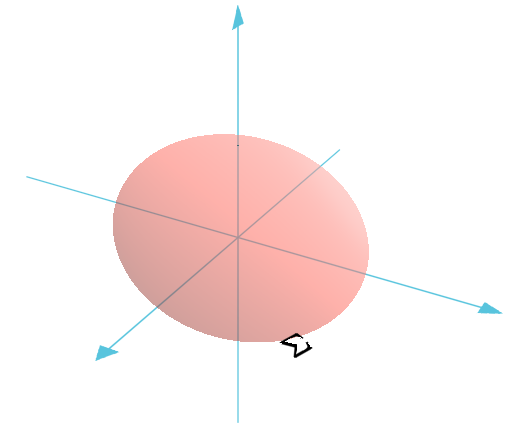
\includegraphics[scale=0.3]{figures/ell1.png}
% \end{figure}

\begin{example}
    求 $\displaystyle I=\iint\limits_\varSigma\dfrac{\dd S}{\qty(x^2+y^2+z^2)^{\frac{3}{2}}\sqrt{\dfrac{x^2}{a^4}+\dfrac{y^2}{b^4}+\dfrac{z^2}{c^4}}}$, 
    其中曲面 $\varSigma$ 是方程 $$\dfrac{x^2}{a^2}+\dfrac{y^2}{b^2}+\dfrac{z^2}{c^2}=1~ (a,b,c>0)$$ 确定的椭球面.
\end{example}
\begin{solution}
    记 $F(x,y,z)=\dfrac{x^2}{a^2}+\dfrac{y^2}{b^2}+\dfrac{z^2}{c^2}-1=0$, 取 $\vec{n}$ 为曲面 $\varSigma$ 指向外侧的法向量, 则\newline
    \begin{minipage}{0.75\linewidth}
        $$\vec{n}=\qty(F'_x,F'_y,F'_z)=\qty(\dfrac{2x}{a^2},\dfrac{2y}{a^2},\dfrac{2z}{a^2})$$
        对应的单位向量, 即方向余弦构成的向量为
        \begin{flalign*}
            \vec{n}^\circ & =\dfrac{1}{\sqrt{\dfrac{4x^2}{a^4}+\dfrac{4y^2}{a^4}+\dfrac{4z^2}{a^4}}}\qty(\dfrac{2x}{a^2},\dfrac{2y}{a^2},\dfrac{2z}{a^2})                              \\
                          & =\dfrac{1}{\sqrt{\dfrac{x^2}{a^4}+\dfrac{y^2}{a^4}+\dfrac{z^2}{a^4}}}\qty(\dfrac{x}{a^2},\dfrac{y}{a^2},\dfrac{z}{a^2})=(\cos \alpha,\cos\beta,\cos\gamma)
        \end{flalign*}
        于是
        \begin{flalign*}
            I & =\iint\limits_\varSigma\dfrac{\dfrac{x^2}{a^2}+\dfrac{y^2}{b^2}+\dfrac{z^2}{c^2}}{\qty(x^2+y^2+z^2)^{\frac{3}{2}}\sqrt{\dfrac{x^2}{a^4}+\dfrac{y^2}{b^4}+\dfrac{z^2}{c^4}}}\dd S=\iint\limits_\varSigma\dfrac{\qty(\dfrac{x}{a^2},\dfrac{y}{b^2},\dfrac{z}{c^2})}{\sqrt{\dfrac{x^2}{a^4}+\dfrac{y^2}{b^4}+\dfrac{z^2}{c^4}}}\cdot\dfrac{(x,y,z)}{\qty(x^2+y^2+z^2)^{\frac{3}{2}}}\dd S \\
              & =\iint\limits_\varSigma\dfrac{x\cos \alpha+y\cos\beta+z\cos\gamma}{\qty(x^2+y^2+z^2)^{\frac{3}{2}}}\dd S=\iint\limits_\varSigma\dfrac{x\dd y\dd z+y\dd z\dd x+z\dd x\dd y}{\qty(x^2+y^2+z^2)^{\frac{3}{2}}}
        \end{flalign*}
    \end{minipage}\hfill
    \begin{minipage}{0.21\linewidth}
        \begin{figure}[H]
            \centering
            \tdplotsetmaincoords{60}{120}
            \begin{tikzpicture}[->,samples=100,>=stealth,tdplot_main_coords,scale=0.65,font=\footnotesize]
                \coordinate (xMin) at ( -2.5,   0,  0);
                \coordinate (xMax) at ( 2.5,    0,  0);
                \coordinate (yMin) at ( 0,  -2.5,   0);
                \coordinate (yMax) at ( 0,  2.5,    0);
                \coordinate (zMin) at ( 0,  0,  -2.5);
                \coordinate (zMax) at ( 0,  0,  2.5);
                \draw[thick,->, cyan] (xMin) -- (0,0,0) node [below right] {$O$} -- (xMax) node[anchor=north east]{$x$};
                \draw[thick,->, cyan] (yMin) -- (0,0,0) -- (yMax) node[anchor=north west]{$y$};
                \draw[thick,->, cyan] (zMin) -- (0,0,0) -- (zMax) node[anchor=south]{$z$};
                \draw[black] (0,0,0) ellipse [x radius=1, y radius=2];
                \begin{scope}[canvas is zy plane at x=0]
                    \draw (0,0) ellipse (1.5 and 2);
                \end{scope}
                \begin{scope}[canvas is zx plane at y=0]
                    \draw (0,0) ellipse (1.5 and 1);
                \end{scope}
                \draw[black,densely dashed] (0,0,0) circle (5pt);
                \filldraw (1,0,0) circle (1pt) (-1,0,0) circle (1pt)
                (0,2,0) circle (1pt) (0,-2,0) circle (1pt)
                (0,0,1.5) circle (1pt) (0,0,-1.5) circle (1pt);
            \end{tikzpicture}
            \caption{}
            \label{dsx2y2z232}
        \end{figure}
    \end{minipage}\newline
    补 $\varSigma_\varepsilon:x^2+y^2+z^2=\varepsilon^2~ (\varepsilon>0)$, 取内侧, $\Omega_\varepsilon$ 是 $\varSigma_\varepsilon$ 所围成立体区域, 因此
    \begin{flalign*}
        I & =\qty(\oiint\limits_{\varSigma+\varSigma_\varepsilon}-\iint\limits_{\varSigma_\varepsilon})\dfrac{x\dd y\dd z+y\dd z\dd x+z\dd x\dd y}{\qty(x^2+y^2+z^2)^{\frac{3}{2}}}=-\iint\limits_{\varSigma_\varepsilon}\dfrac{x\dd y\dd z+y\dd z\dd x+z\dd x\dd y}{\qty(x^2+y^2+z^2)^{\frac{3}{2}}} \\
          & =-\dfrac{1}{\varepsilon^2}\iint\limits_{\varSigma_\varepsilon}x\dd y\dd z+y\dd z\dd x+z\dd x\dd y=\dfrac{3}{\varepsilon^3}\iiint\limits_{\Omega_\varepsilon}\dd V=\dfrac{3}{\varepsilon^3}\cdot\dfrac{4}{3}\pi\varepsilon^3=4\pi.
    \end{flalign*}
\end{solution}

\begin{example}
    (第十一届数学竞赛决赛) 设 $\Omega$ 是由光滑简单封闭曲面 $\varSigma$ 围成的有界闭区域, 函数 $f(x,y,z)$ 在 $\Omega$ 上具有连续二阶导数, 且 $f(x,y,z)|_{(x,y,z)\in\varSigma}=0$, 记 $\nabla f$ 为 $f(x,y,z)$ 的梯度, 并令
    $$\Delta f=\frac{\partial^2 f}{\partial x^2}+\frac{\partial ^2f}{\partial y^2}+\frac{\partial ^2f}{\partial z^2},~$$
    证明, 对任意常数 $C>0$, 恒有
    $$C\iiint\limits_\Omega f^2\dd x\dd y\dd z+\frac{1}{C}\iiint\limits_\Omega(\Delta f)^2\dd x\dd y\dd z\geqslant2\iiint\limits_\Omega|\nabla f|^2\dd x\dd y\dd z$$
\end{example}
\begin{proof}[{\songti \textbf{证}}]
    由 Gauss 公式, 得
    $$\oiint\limits_\varSigma f\frac{\partial f}{\partial x}\dd y\dd z+f\frac{\partial f}{\partial y}\dd z\dd x+f\frac{\partial f}{\partial x}\dd x\dd y=\iiint\limits_\Omega\left(f\Delta f+|\nabla f|^2\right)\dd x\dd y\dd z$$
    因为 $f(x,y,z)|_{(x,y,z)\in \varSigma}=0$, 所以上式左端等于 0.
    \begin{flalign*}
        \iiint\limits_\Omega|\nabla f|^2\dd x\dd y\dd z=-\iiint\limits_\Omega f\Delta f \dd x\dd y\dd z
        \leqslant\left(\iiint\limits_\Omega f^2\dd x\dd y\dd z\right)^{\frac{1}{2}}\left(\iiint\limits_\Omega(\Delta f)^2\dd x\dd y\dd z\right)^{\frac{1}{2}}
    \end{flalign*}
    故对任意的 $C$ 均有, 
    \begin{flalign*}
        C\iiint\limits_\Omega f^2\dd x\dd y\dd z+\frac{1}{C}\iiint\limits_\Omega(\Delta f)^2\dd x\dd y\dd z
         & \geqslant2\left(\iiint\limits_\Omega f^2\dd x\dd \dd z\right)^{\frac{1}{2}}\left(\iiint\limits_\Omega(\Delta f)^2\dd x\dd y\dd z\right)^{\frac{1}{2}}
        \geqslant2\iiint\limits_\Omega|\nabla f|^2\dd x\dd y\dd z
    \end{flalign*}
\end{proof}

\begin{example}
    设 $f(x,y,z)$ 在 $\varSigma$ 上的连续函数, 且满足
    $$f(x,y,z)=(x+y+z)^2+\iint\limits_\varSigma f(x,y,z)\dd y\dd z+x^2\dd x\dd y$$
    其中 $\varSigma:x^2+y^2=5z~ (0\leqslant z\leqslant 1)$, 方向为下侧, 求 $f(x,y,z)$ 的表达式.
\end{example}
\begin{solution}
    令 $\displaystyle\iint\limits_\varSigma f(x,y,z)\dd y\dd z=A$, 并且
    \begin{flalign*}
        \iint\limits_\varSigma x^2\dd x\dd y=-\iint\limits_{x^2+y^2\leqslant 5}x^2\dd x\dd y=-\int_{0}^{2\pi}\dd \theta\int_{0}^{\sqrt{5}}\rho^2\cos^2\theta\rho\dd \rho=-\dfrac{25\pi}{4}
    \end{flalign*}
    于是, $f(x,y,z)=(x+y+z)^2+A-\dfrac{25\pi}{4}$, 两边积分得
    $$A=\iint\limits_\varSigma f(x,y,z)\dd y\dd z=\iint\limits_{\varSigma}\qty[(x+y+z)^2+A-\dfrac{25\pi}{4}]\dd y\dd z$$
    添加一平面 $\varSigma_1:z=1,x^2+y^2\leqslant 5$, 方向取上侧, 则由 Gauss 公式
    \begin{flalign*}
        \oiint\limits_{\varSigma+\varSigma_1}\qty[(x+y+z)^2+A-\dfrac{25\pi}{4}]\dd y\dd z & =\iiint\limits_{\Omega}2(x+y+z)\dd V=2\iiint\limits_\Omega z\dd V
        =2\int_{0}^{2\pi}\dd \theta\int_{0}^{\sqrt{5}}r\dd r\int_{\frac{r^2}{5}}^{1}z\dd z=\dfrac{10\pi}{3}
    \end{flalign*}
    且 $\displaystyle\iint\limits_{\varSigma_1}\qty[(x+y+z)^2+A-\dfrac{25\pi}{4}]\dd y\dd z=0$, 所以 $A=\dfrac{10\pi}{3}$, 
    于是 $f(x,y,z)=(x+y+z)^2-\dfrac{35}{12}\pi.$
\end{solution}

\subsubsection{Stokes 公式}

\begin{theorem}[Stokes 积分法]
    设 $ \varSigma $ 是逐段光滑的单闭曲线 $ \Gamma $ 所包围的非封闭光滑双侧曲面, 取某定侧 $ \varSigma^{+} $, 按右手规则确定 $ \Gamma $ 的正向 $ \Gamma^{+}$, $\Omega $
    是空间的立体区域, 使得 $ \varSigma \subset \Omega $, 函数 $P,~  Q,~ R$ 在 $ \Omega $ 上连续可微, 则有 Stokes 公式:
    \begin{flalign*}
          & \oint_{\Gamma^{+}} P(x, y, z) \dd  x+Q(x, y, z) \dd  y+R(x, y, z) \dd  z                                                                                                                                                                                                                         \\
        = & \iint\limits_{\varSigma^{+}}\left(\frac{\partial R}{\partial y}-\frac{\partial Q}{\partial z}\right) \dd  y \dd  z+\left(\frac{\partial P}{\partial z}-\frac{\partial R}{\partial x}\right) \dd  z \dd  x+\left(\frac{\partial Q}{\partial x}-\frac{\partial P}{\partial y}\right) \dd  x \dd  y \\
        = & \iint\limits_{\varSigma^{+}}\begin{vmatrix}
                                            \dd y\dd z            & \dd z\dd x            & \dd x\dd y            \\
                                            \displaystyle \pdv{x} & \displaystyle \pdv{y} & \displaystyle \pdv{z} \\
                                            P                     & Q                     & R
                                        \end{vmatrix}
        =\iint\limits_{\varSigma^{+}}\begin{vmatrix}
                                         \cos\alpha            & \cos\beta             & \cos\gamma            \\
                                         \displaystyle \pdv{x} & \displaystyle \pdv{y} & \displaystyle \pdv{z} \\
                                         P                     & Q                     & R
                                     \end{vmatrix}\dd S
    \end{flalign*}
    \index{Stokes 积分法}
\end{theorem}

\begin{theorem}
    空间曲线积分与路径无关的充要条件: 设 $ G $ 是空间的面单连通区域, 函数 $ P, Q, R $ 在 $ G $ 上连续可微, 则下列四条陈述相互等价:
    \begin{enumerate}[label=(\arabic{*})]
        \item $\forall(x, y, z) \in \Omega$, $\dfrac{\partial R}{\partial y}=\dfrac{\partial Q}{\partial z}$, 
              $\dfrac{\partial P}{\partial z}=\dfrac{\partial R}{\partial x}$, $\dfrac{\partial Q}{\partial x}=\dfrac{\partial P}{\partial y} $;
        \item $\forall A, B \in \Omega$, $\displaystyle \int_{A}^{B} P \dd  x+Q \dd  y+R \dd  z $ 与路线无关;
        \item $\forall \Gamma \subset \Omega$, $\Gamma $ 为封闭曲线, $\displaystyle \oint_{\Gamma} P \dd  x+Q \dd  y+R \dd  z=0 $;
        \item  存在可微函数 $ u(x, y, z) $, 使得 $ \dd  u=P \dd  x+Q \dd  y+R \dd  z $, 且
              $$u(x, y, z)=\int_{x_{0}}^{x} P\left(x, y_{0}, z_{0}\right) \dd  x+\int_{y_{0}}^{y} Q\left(x, y, z_{0}\right) \dd  y+\int_{z_{0}}^{z} R(x, y, z) \dd  z+C$$
              或
              $$u(x, y, z)=\int_{x_{0}}^{x} P(x, y, z) \dd  x+\int_{y_{0}}^{y} Q\left(x_{0}, y, z\right) \dd  y+\int_{z_{0}}^{z} R\left(x_{0}, y_{0}, z\right) \dd  z+C$$
              这里 $ \left(x_{0}, y_{0}, z_{0}\right),(x, y, z) \in G $.
    \end{enumerate}
\end{theorem}

\begin{example}
    计算 $\displaystyle I=\int_{\Gamma}(y-z)\dd x+(z-x)\dd y+(x-y)\dd z$, 其中 $\Gamma$ 是柱面 $x^2+y^2=R^2$ 和平面 $x+z=R$ 相交的椭圆, 且从 $x$ 轴正向看去, $\Gamma$ 的方向是逆时针的.
\end{example}
\begin{solution}
    设 $\Sigma$ 为平面 $x+y=R$ 被柱面截下部分的上侧, 则由 Stokes 公式, 有
    \begin{flalign*}
        I & =\iint\limits_\Sigma\begin{vmatrix}
                                    \dd y\dd z                                & \dd z\dd x                                & \dd x\dd y                                \\
                                    \displaystyle\frac{\partial }{\partial x} & \displaystyle\frac{\partial }{\partial y} & \displaystyle\frac{\partial }{\partial z} \\
                                    P                                         & Q                                         & R
                                \end{vmatrix}=\iint\limits_\Sigma-2\dd y\dd z-2\dd z\dd x-2\dd x\dd y \\
          & =-2\iint\limits_{D_{yz}}\dd y\dd z-2\iint\limits_{D_{zx}}\dd z\dd x-2\iint\limits_{D_{xy}}\dd x\dd y=-2\pi R^2-0-2\pi R^2=-4\pi R^4.
    \end{flalign*}
\end{solution}

\begin{example}[第九届数学竞赛预赛]
    设曲线 $\Gamma$ 为在 $x^2+y^2+z^2=1$, $x+z=1$, $x\geqslant0$, $y\geqslant0$, $z\geqslant0$ 上从 $A(1,0,0)$ 到 $B(0,0,1)$ 的一段, 求 $\displaystyle I=\oint_\Gamma y\dd x+z\dd y+x\dd z.$
\end{example}
\begin{solution}
    记 $\Gamma_1$ 为 $B$ 到 $A$ 的直线段, 则
    $$x=t,y=0,z=1-t,0\leqslant t\leqslant1$$
    $$\int_{\Gamma_1}y\dd x+z\dd y+x\dd z=\int_0^1t\dd (1-t)=-\frac{1}{2}$$
    \begin{flalign*}
        \oint_{\Gamma+\Gamma_1}y\dd x+z\dd y+x\dd z & =\iint\limits_\Sigma\begin{vmatrix}
                                                                              \dd y\dd z                                & \dd z\dd x                                & \dd x\dd y                                \\
                                                                              \displaystyle\frac{\partial }{\partial x} & \displaystyle\frac{\partial }{\partial y} & \displaystyle\frac{\partial }{\partial z} \\[6pt]
                                                                              P                                         & Q                                         & R
                                                                          \end{vmatrix}=\iint\limits_\Sigma-\dd x\dd y-\dd z\dd x-\dd y\dd z \\
                                                    & =-\iint\limits_{D_{xy}}\dd x\dd y-\iint\limits_{D_{zx}}\dd z\dd x-\iint\limits_{D_{yz}}\dd y\dd z
        =-\frac{\pi}{2\sqrt{2}}
    \end{flalign*}
    $$I=\oint_{\Gamma+\Gamma_1}-\int_{\Gamma_1}=\oint_{\Gamma}y\dd x+z\dd y+x\dd z=\frac{1}{2}-\frac{\pi}{2\sqrt{2}}.$$
\end{solution}

\begin{example}[2001 数一]
    计算 $$I=\oint_L\qty(y^2-z^2)\dd x+\qty(2z^2-x^2)\dd y+\qty(3x^2-y^2)\dd z$$
    其中 $L$ 是平面 $x+y+z=2$ 与柱面 $|x|+|y|=1$ 的交线, 从 $z$ 轴正方向看去, $L$ 为逆时针方向.
\end{example}
\begin{solution}
    设 $\varSigma$ 为平面 $x+y+z=2$ 的上侧被 $L$ 所围成的部分, $\varSigma$ 在 $xOy$ 面的投影区域为
    $$D_{xy}=\{(x,y)|~|x|+|y|\leqslant 1\}$$
    $\varSigma$ 的单位向量为 $\dfrac{1}{\sqrt{3}}\{1,1,1\}$, 于是由 Stokes 公式得
    \begin{flalign*}
        I & =\iint\limits_\varSigma\begin{vmatrix}
                                       \dfrac{1}{\sqrt{3}}   & \dfrac{1}{\sqrt{3}}   & \dfrac{1}{\sqrt{3}}   \\[6pt]
                                       \displaystyle \pdv{x} & \displaystyle \pdv{y} & \displaystyle \pdv{z} \\[6pt]
                                       y^2-z^2               & 2z^2-x^2              & 3x^2-y^2
                                   \end{vmatrix}\dd S
        =-\dfrac{2}{\sqrt{3}}\iint\limits_\varSigma(4x+2y+3z)\dd S                                                                                    \\
          & =-\dfrac{2}{\sqrt{3}}\iint\limits_{D_{xy}}(x-y+6)\sqrt{1+(z'_x)^2+(z'_y)^2}\dd x\dd y=-2\iint\limits_{D_{xy}}(x-y+6)\dd x\dd y
    \end{flalign*}
    由二重积分的对称性知 $\displaystyle\iint\limits_{D_{xy}}(x-y)\dd x\dd y=0$, 所以 $\displaystyle I=-12\iint\limits_{D_{xy}}\dd x\dd y=-24.$
\end{solution}

\begin{example}
    求曲线积分 $$I=\oint_L(y-z)\dd x+(z-x)\dd y+(x-y)\dd z$$
    其中 $L$ 是两球面 $$x^2+y^2+z^2=1~  (x-1)^2+(y-1)^2+(z-1)^2=4$$
    的交线, 积分方向从 $z$ 轴正向看为逆时针方向.
\end{example}
\begin{solution}
    由 $\displaystyle \left\{\begin{matrix}
            x^2     & + & y^2     & + & z^2     & =1 \\
            (x-1)^2 & + & (y-1)^2 & + & (z-1)^2 & =4
        \end{matrix}\right.\Rightarrow x+y+z=0$, 平面 $x+y+z=0$ 上, 曲线 $L$ 所包围的圆域为 $\varSigma$, 即 $$\varSigma=\{(x,y,z)|x+y+z=0,x^2+y^2+z^2\leqslant 1\}$$
    于是, 由 Stokes 公式得
    \begin{flalign*}
        I & =\iint\limits_\varSigma\begin{vmatrix}
                                       \cos\alpha            & \cos\beta             & \cos\gamma            \\
                                       \displaystyle \pdv{x} & \displaystyle \pdv{y} & \displaystyle \pdv{z} \\
                                       y-z                   & z-x                   & x-y
                                   \end{vmatrix}\dd S=-2\iint\limits_\varSigma(\cos\alpha+\cos\beta+\cos\gamma)\dd S \\
          & =-\dfrac{6}{\sqrt{3}}\iint\limits_\varSigma\dd S=-\dfrac{6}{\sqrt{3}}\cdot\pi\cdot 1^2=-2\sqrt{3}\pi.
    \end{flalign*}
\end{solution}

\begin{example}
    设 $L$ 为空间某封闭光滑曲线, $P,~Q,~R$ 为空间中具有一阶连续偏导数的函数, 证明:
    $$\qty|\oint_{L^+}P\dd x+Q\dd y+R\dd z|\leqslant \max\limits_{(x,y,z)\in S}\sqrt{\qty(\pdv{Q}{x}-\pdv{P}{y})^2+\qty(\pdv{R}{y}-\pdv{Q}{z})^2+\qty(\pdv{P}{z}-\pdv{P}{x})^2}\cdot S$$
    其中 $S$ 表示 $L$ 上展开的 (以 $L$ 为边界的) 某曲面, 同时也用它表示曲面的面积.
\end{example}
\begin{proof}[{\songti \textbf{证}}]
    由 Cauchy-Schwarz 不等式, 
    \begin{flalign*}
        \text{左端} & \xlongequal[]{\text{Stokes}}\iint\limits_S\qty[(R_y'-Q_z')\cos\alpha+(P_z'-R_x')\cos\beta+(Q_x'-P_y')\cos\gamma]\dd S           \\
                    & \leqslant \iint\limits_S\sqrt{\qty[(R_y'-Q_z')^2+(P_z'-R_x')^2+(Q_x'-P_y')^2]\cdot(\cos^2\alpha+\cos^2\beta+\cos^2\gamma)}\dd S \\
                    & \leqslant \max\limits_{(x,y,z)\in S}\sqrt{(R_y'-Q_z')^2+(P_z'-R_x')^2+(Q_x'-P_y')^2}\cdot\iint\limits_S\dd S=\text{右端}
    \end{flalign*}
\end{proof}

\begin{example}
    设 $f(x)$ 一阶连续可导, $$R(x,y,z)=\int_{0}^{x^2+y^2}f(z-t)\dd t$$
    曲面 $\varSigma$ 为抛物面 $z=x^2+y^2$ 被平面 $y+z=1$ 所截的下面部分的内侧, $L$ 为 $\varSigma$ 的正向边界, 求
    $$I=\oint_L2xzf\qty(z-x^2-y^2)\dd x+\qty[x^3+2yzf\qty(z-x^2-y^2)]\dd y+R(x,y,z)\dd z.$$
\end{example}
\begin{proof}[{\songti \textbf{证}}]
    记 $P(x,y,z)=2xzf\qty(z-x^2-y^2),~Q(x,y,z)=x^3+2yzf\qty(z-x^2-y^2)$, 则
    $$\pdv{P}{y}=-4xyzf'\qty(z-x^2-y^2),~\pdv{P}{z}=2x\qty(f\qty(z-x^2-y^2)+zf'\qty(z-x^2-y^2))$$
    $$\pdv{Q}{x}=3x^2-4xyzf'\qty(z-x^2-y^2),~\pdv{Q}{z}=2y\qty(f\qty(z-x^2-y^2)+zf'\qty(z-x^2-y^2))$$
    令 $u=z-t$, 则 $\dd t=-\dd u$, 于是 $\displaystyle R(x,y,z)=\int_{z-x^2-y^2}^{z}f(u)\dd u$, 
    $$\pdv{R}{x}=\pdv{x}\qty(\int_{z-x^2-y^2}^{z}f(u)\dd u)=2xf\qty(z-x^2-y^2),~\pdv{R}{y}=2yf\qty(z-x^2-y^2)$$
    于是
    \begin{flalign*}
        \pdv{R}{y}-\pdv{Q}{z} & =-2yzf'\qty(z-x^2-y^2)=-2yzf'(0) \\
        \pdv{P}{z}-\pdv{R}{x} & =2xzf'\qty(z-x^2-y^2)=2xzf'(0)   \\
        \pdv{Q}{x}-\pdv{P}{y} & =3x^2
    \end{flalign*}
    则由 Stokes 公式知, 
    \begin{flalign*}
        I & =\iint\limits_\varSigma\left(\frac{\partial R}{\partial y}-\frac{\partial Q}{\partial z}\right) \dd  y \dd  z+\left(\frac{\partial P}{\partial z}-\frac{\partial R}{\partial x}\right) \dd  z \dd  x+\left(\frac{\partial Q}{\partial x}-\frac{\partial P}{\partial y}\right) \dd  x \dd  y \\
          & =\iint\limits_\varSigma-2yzf'(0)\dd y\dd z+2xzf'(0)\dd z\dd x+3x^2\dd x\dd y
    \end{flalign*}
    补面 $\varSigma_1:\begin{cases}
            y+z=1 \\
            z=x^2+y^2
        \end{cases}$, 方向取下侧, 由 Gauss 公式可知, 
    \begin{flalign*}
        I & =\qty(\oiint\limits_{\varSigma+\varSigma_1}-\iint\limits_{\varSigma_1})\qty(-2yzf'(0)\dd y\dd z+2xzf'(0)\dd z\dd x+3x^2\dd x\dd y)                                 \\
          & =-\iint\limits_{\varSigma_1}\qty(-2yzf'(0)\dd y\dd z+2xzf'(0)\dd z\dd x+3x^2\dd x\dd y)=3\iint\limits_{x^2+\qty(y+\frac{1}{2})^2\leqslant\frac{5}{4}}x^2\dd x\dd y
    \end{flalign*}
    令 $\begin{cases}
            x=\dfrac{\sqrt{5}}{2}\rho\cos\theta \\[6pt]
            y=\dfrac{\sqrt{5}}{2}\rho\sin\theta-\dfrac{1}{2}
        \end{cases}$, 于是 $\displaystyle\pdv{(x,y)}{(\rho,\theta)}=\dfrac{5}{4}\rho$, 所以
    $\displaystyle I=3\int_{0}^{2\pi}\dd \theta\int_{0}^{1}\dfrac{5}{4}\rho^2\cos^2\theta\dfrac{5}{4}\rho\dd \rho=\dfrac{75\pi}{64}.$
\end{proof}

% \subsection{Ostrogradsky 公式}

% \begin{theorem}[Ostrogradsky 定理]
%     若空间区域 $V$ 的边界 $S$ 为分片光滑曲面, $P=P(x,y,z),~Q=Q(x,y,z),~R=R(x,y,z)$ 和它们的一阶偏导数均在区域 $V+S$ 内的连续函数, 
%     则 $$\iint\limits _{S}\left( P\cos \alpha +Q\cos \beta +R\cos \gamma \right) \dd S=\iiint\limits _{V}\left( \dfrac{\partial P}{\partial x}+\dfrac{\partial Q}{\partial y}+\dfrac{\partial R}{\partial z}\right) \dd x\dd y\dd z.$$
%     式中 $\cos\alpha,~\cos\beta,~\cos\gamma$ 为曲面 $S$ 的外法线的方向余弦.
% \end{theorem}
